\chapter{Método utilizando los acoplamientos mutuos}
\label{ch:estado}
\lhead{\emph{Método utilizando los acoplamientos mutuos}}

Una antena se calibra buscando que no solo todos los caminos de recepción atenúen y defasen exactamente lo mismo, sino que 
también sea un valor conocido. Para transmisión se busca lo mismo, con la salvedad que se puede modificar la fase de la 
señal que se emite en algunos RMs para modificar el lugar de apuntamiento de la antena.

Hay distintos factores que hacen que los componentes dejen de comportarse de forma nominal, por ejemplo se puede nombrar el
cambio de temperatura, el mero envejecimiento de los componentes al pasar el tiempo, que un mero cable se haya doblado más
de la cuenta, interferencias electromagnéticas, radiadas o conducidas, o entre distintos componentes, etc. 

Es importante que un patrón de antena posea los lóbulos secundarios lo más chicos posibles con respecto al lóbulo principal,
que el lóbulo principal sea lo más angosto posible, con esto se aumenta la resolución espacial. Un factor que ocurre es el 
de los targets ficticios.\todo{no se como se elimina}


\todo{poner que factores hacen que cambie la ganancia de los componentes para calibrar la antena}
\todo{poner que ocurre con el antnena pattern si no está correctamente calibrada, altura de lóbulos secundarios, ancho 
de lóbulo principal, pico del lóbulo principal, etc}

Para poder calibrar esta antena polarimétrica haciendo uso de los acoplamientos mutuos, se cuenta con el uso de 
cuadrados mínimos. La idea es realizar lazos de calibración transmitiendo en una polarización y recibiendo en la
otra a la vez. Para esto, es necesario que no solo se pueda configurar algunos RMs em modo $T_x$ y otros en modo $R_x$ en 
distintas polarizaciones, sino también poder configurar los módulos que no forman parte de dicho lazo en modo alta 
impedancia (en este modo el módulo no transmite ni recibe nada, evitando así la inyección de ruido y señal en zonas 
indeseadas de la antena). 

Tomando como caso una antena rectangular de $M x N$ módulos radiantes y asumiendo que solo se transmite y recibe de a un 
RM por lazo de calibración, a priori, se dispone de un máximo de $(MN)^2$ ecuaciones. La cantidad de incógnitas de todos
los caminos de la RFDN, tanto transmisión como recepción en ambas polarizaciones (H y V), son $4MN$. A su vez, en el 
apéndice \ref{AppendixA} se realiza el cálculo de la cantidad de acoplamientos mutuos que posee una antena polarimétrica,
particularmente, la ecuación \ref{eq:amountMutCoupling} muestra la cantidad de incógnitas, que, para este caso, resulta 
ser de $MN(MN-1)/2$. Totalizando en $MN(MN + 7)/2$ incógnitas.

Para que el sistema tenga solución, la cantidad de ecuaciones debe ser mayor que la de incógnitas. Esta restricción solo 
se cumple si se calibra toda la antena en un solo paso (Tx y Rx en ambas polarizaciones) porque es el único caso en que 
cada acoplamiento mútuo aparezca más de una única vez. En caso contrario, habrían siempre más incógnitas que ecuaciones.

\todo{tener en cuenta que por ahora el requerimiento es que la antena sea totalmente plana}

\begin{comment}

Una vez definido el modelo matemático que se pretende emular y el soporte físico sobre el cuál ejecutarlo, se procede a la aplicación del instrumento
que permitirá enlazar las dos partes del proyecto: el control.

Los sistemas de control constituyen una herramienta muy poderosa para la resolución de problemas en ingeniería. Las técnicas que proporciona son de
esencial importancia para el diseño de sistemas complejos. En electrónica, la aplicación de los recursos que proporciona el control automático son
ampliamente utilizados y cada vez encuentran más aplicaciones y de mejor desempeño, gracias al avance de los sistemas embebidos en los últimos tiempos.

Los sistemas digitales modernos han ofrecido un soporte muy robusto a la teoría de control, posibilitando la implementación de funciones y técnicas
que de otro modo serían impracticables. El uso de las herramientas de control mediante sistemas embebidos tiene la gran ventaja, frente a 
mecanismos analógicos, de ser realizados por medio de la programación de los algoritmos que definen la operación a efectuar, de modo que permiten
gran libertad y rigidez al diseño.

Los equipos de potencia electrónicos tienen grandes exigencias temporales para la operación que realizan, tal es el caso de los convertidores conmutados
que requieren de una razonable velocidad de conmutación de las llaves electrónicas que los componen. Es por ello que la electrónica de potencia recibe una
ayuda indispensable del control de sistemas discretos.

El \emph{hardware} utilizado consiste en un DSP que posee varios módulos, de los cuales varios han sido utilizados tanto para hacer cálculos, relevar
mediciones o entregar señales de control. La programación ha sido realizada progresivamente por medio de dos entornos de programación, uno de nivel más
alto y otro de más bajo nivel que contiene el compilador del código que es programado directamente en el dispositivo.

Este capítulo presenta la teoría utilizada para la realización de del trabajo así como los modelos completos de los sistemas implementados. Los elementos
explicados y utilizados van desde filtros digitales hasta controladores elementales y el promediado de sistemas de estructura variable.

\section{Introducción}
Existen diversas opciones al momento de aplicar una estrategia de control a un sistema dado, y además muchas de éstas vienen combinadas entre sí. Para el
abordaje del problema del control de un sistema se establecen ciertos procedimientos que involucran la gestión de la información tomada del sistema (medidas,
modelos, por ejemplo) y el modo en que las acciones de control interactúan con el sistema mencionado. La disposición de estas interacciones es la arquitectura
de control.

La disposición más común en la arquitectura de control, es sin duda la realimentación. Este es un concepto fundamental de la teoría de control y ofrece una multitud
de mejoras al desempeño de los sistemas si ha sido correctamente empleada. Su principio subyace en que a pesar de no conocer con precisión la naturaleza del 
sistema que se controla, se realizan correcciones en las acciones de control utilizando la información medida del efecto que produce el ajuste de sus variables de entrada.

La realimentación puede darse de varias maneras, aunque la aplicación más sencilla consiste en simplemente en obtener la diferencia entre la variable que se 
desea controlar y cierta referencia. A este resultado se le llama error, y dado que la magnitud medida se resta a la referencia, la realimentación es negativa.
El valor del error puede ser utilizado directamente como variable de control o bien puede incorporarse un controlador para procesar esa información y obtener
así otro comportamiento.

\section{Controladores}

Para el control de los sistemas lineales, una elección típica para del controlador es la de los PID (Proporcional Integral y Derivativo) que constituyen los 
más utilizados en el mundo del control. La acción que realizan se obtiene a partir del error entre la referencia que se pretende seguir y la medición
de la variable que se pretende controlar. Las acciones que realizan los PID se componen fundamentalmente de tres operaciones: la acción \emph{proporcional} que
considera el valor actual del error obtenido; la acción \emph{integral} que tiene en cuenta las contribuciones de las mediciones previas; y por último
la acción \emph{derivativa} que realiza una predicción de los valores futuros del error. Esta idea se ilustra en la fig. \ref{fig:accion_PID}. Cada uno
de estos cálculos están acompañados por ciertos parámetros.

\begin{figure}
 \centering
 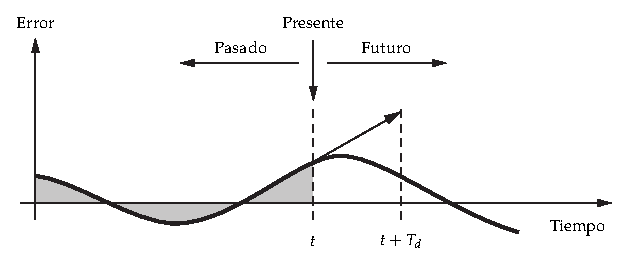
\includegraphics[width=10cm]{gfx/accion_PID}
 \caption{Consideración del controlador PID a los valores obtenidos.}
 \label{fig:accion_PID}
\end{figure}

Los efectos de las operaciones que componen al controlador PID tienen un propósito distinto, es decir que son complementarias. Esto se explica a continuación
\begin{itemize}
 \item \textbf{Acción Proporcional}: Aumenta la velocidad en la que se modifica la respuesta del sistema y disminuye el error de estado estacionario a medida
 que se aumenta.
 \item \textbf{Acción Integral}: Se encarga de eliminar por completo el error de estado estacionario aunque reduce la velocidad a la que responde el sistema.
 La operación matemática es devolver la integral de los valores acumulados del error medido y es por ello que si devuelve un valor constante, quiere decir que
 el error se ha corregido por completo. Una combinación entre las acciones proporcional e integral puede resultar un controlador apropiado en muchos casos 
 y es por ello que es muy común encontrar controladores compuestos únicamente por estas dos acciones.
 \item \textbf{Acción Derivativa}: La idea de esta operación es obtener una anticipación del valor del error a través de la derivada del error realizando una
 corrección prematura, aumentando la velocidad del sistema. Es necesario que el ajuste de los parámetros sean correctamente elegidos para que ésta acción no
 cause comportamientos no deseados, ya que una sintonía inadecuada puede empeorar la estabilidad del sistema generando grandes oscilaciones.
\end{itemize}

Para el control de los convertidores la acción derivativa no es una buena elección debido al rizado causado por la conmutación de las llaves,
lo cual puede considerarse una fuerte perturbación cuyo efecto se vería amplificado. Es por ello que para el proyecto se decidió utilizar un controlador
proporcional e integral, puesto que lo más importante es que el convertidor controlado sea capaz de seguir correctamente las referencias y de momento
no hay necesidad de ampliar el ancho de banda.

Aunque los controladores PID son pensados como módulos de control lineales es razonable considerar la inclusión de ciertos mecanismos no lineales a su diseño.
Esto es debido a que todos los actuadores tienen limitaciones, es decir que a pesar de que la acción de control le exija un comportamiento fuera de sus límites
dicho actuador será conducido a la saturación. Cuando el actuador entra en saturación, el error comienza a crecer y la acción integral también crece sin poder
corregir el error. Si el sistema logra restablecerse fuera de la saturación lo hará luego de largos transitorios, ya que se necesita que el error sea muy
grande y opuesto al valor en que se encuentra saturado el sistema para que el integrador reduzca el valor devuelto, y esto puede conducir nuevamente
a la saturación en otro de los extremos del actuador generando un comportamiento oscilatorio y lento. El efecto explicado se se conoce en la jerga como
\emph{wind-up}. Si se consideran los efectos de la saturación de los actuadores en los algoritmos de control puede evitarse o reducirse su efecto. Esto se logra
agregando un mecanismo que impida que el integrador siga aumentando el valor devuelto una vez que se considere saturado al sistema. Esto se llama
\emph{anti-wind-up} y un ejemplo de implementación se muestra en la fig. \ref{fig:PI_anti-wind-up}.

\begin{figure}
 \centering
 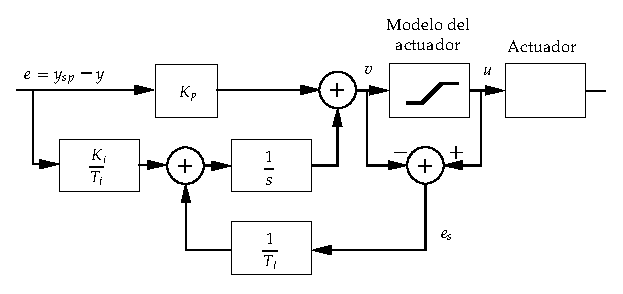
\includegraphics[width=10cm]{gfx/PI_anti-wind-up.eps}
 \caption{Controlador PI con mecanismo anti-wind-up}
 \label{fig:PI_anti-wind-up}
\end{figure}

Los controladores PID suelen ser siempre apropiados para operar sistemas lineales invariantes en el tiempo y es a partir de los modelos que caracterizan dichos
sistemas, como se sintonizan los parámetros de dichos controladores. Para este proyecto los convertidores de potencia no forman parte de estos sistemas debido
a que su estructura cambia según el estado de los transistores de conmutación. Es por ello que se necesita obtener un modelo equivalente para caracterizarlos,
y que sirvan a la sintonía de dichos parámetros.

\section{Modelos promediados de los convertidores}
En el cap. \ref{ch:convertidores} se presentaron los modelos dinámicos de los dos convertidores utilizados en el trabajo. Dado que estos están presentados en
función de la variable de conmutación $u(t)$ es necesario obtener una aproximación del modelo que lo deje expresado de la forma 
$\mathbf{\dot{x}}=\mathbf{Ax}+\mathbf{Bu}$ que definen los sistemas lineales. El procedimiento utilizado es el de promediado de modelo de estados.

El desarrollo siguiente muestra como obtener este modelo, que luego será utilizado para diseñar el controlador con el fin de que el sistema funcione dentro 
de sus márgenes de estabilidad. El procedimiento se muestra a continuación para el caso general que será aplicado al modelo de cada convertidor particular más
adelante.

\begin{equation}
\begin{cases}
\mathbf{\dot{x}_{1}}=\mathbf{A_{1}x}+\mathbf{B_{1}u} & 0<t<dT\\
\mathbf{\dot{x}_{2}}=\mathbf{A_{2}x}+\mathbf{B_{2}u} & dT<t<T
\end{cases}\label{eq:modelo_estados_general}
\end{equation}
\begin{equation}
\begin{cases}
\mathbf{y_{1}}=\mathbf{C_{1}x} & 0<t<dT\\
\mathbf{y_{2}}=\mathbf{C_{2}x} & dT<t<T
\end{cases}\label{eq:transf_lineal}
\end{equation}

Donde el ciclo de trabajo $d$ varía en cada periodo con el tiempo ($d(t)$), según la acción de control. En el segundo sistema matricial
se presenta la transformación lineal que llevará las variables de estado del modelo planteado a las variables de interés. Resolviendo
(\ref{eq:transf_lineal}) para $\mathbf{x}$ y sustituyendo en (\ref{eq:modelo_estados_general}) se obtienen un nuevo espacio de estados
en función de las variables de interés las variables de salida buscada con $\mathbf{A_{yi}}=\mathbf{CA_{i}C^{-1}}$ y $\mathbf{B_{yi}}=\mathbf{CB_{i}}$.
Luego se Parametriza con $u_{d}(t)$,

\begin{equation}
\mathbf{\dot{y}}=(\mathbf{A_{y1}}u_{d}(t)+\mathbf{A_{y2}}(1-u_{d}(t)))\mathbf{y}+(\mathbf{B_{y1}}u_{d}(t)+\mathbf{B_{y2}}(1-u_{d}(t)))\mathbf{u}
\end{equation}
$$u_{d}(t)=\begin{cases}
1, & 0<t<dT\\
0, & dT<t<T
\end{cases}$$
Realizando un promedio temporal (por periodo) del sistema,
\begin{equation}
\langle\mathbf{\dot{y}}\rangle(t)=(\mathbf{A_{y1}}d(t)+\mathbf{A_{y2}}(1-d(t)))\langle\mathbf{y}\rangle(t)+(\mathbf{B_{y1}}d(t)+\mathbf{B_{y2}}(1-d(t)))\langle\mathbf{u}\rangle(t)
\label{eq:promediada}
\end{equation}
Y linealizando el sistema alrededor de un punto de trabajo supuesto (considerando pequeñas variaciones alrededor de éste último),
\begin{equation}
\langle\mathbf{y}\rangle(t)=\mathbf{\bar{y}}+\mathbf{\tilde{y}}(t)\label{eq:linealizacionx}
\end{equation}
\begin{equation}
d(t)=\bar{d}+\tilde{d}(t)\label{eq:linealizaciond}
\end{equation}
Es posible obtener las funciones de transferencia de cada variable de estado respecto de la variable de control promediada $u_{d}(t)$, es decir $\tilde{d}(t)$,
\begin{equation}
\mathbf{T}(s)=\left(\begin{array}{c}
\frac{I_{L}(s)}{d(s)}\\
\frac{U_{o}(s)}{d(s)}
\end{array}\right)
\end{equation}
Usando (\ref{eq:linealizacionx}) y (\ref{eq:linealizaciond}) en (\ref{eq:promediada}) y reordenando:
\begin{eqnarray}
\mathbf{\dot{\tilde{y}}}(t)=((\mathbf{A_{y1}}\bar{d}+\mathbf{A_{y2}}(1-\bar{d}))+ (\mathbf{A_{y1}}-\mathbf{A_{y2}})\tilde{d}(t))(\mathbf{\bar{y}}+\mathbf{\tilde{y}}(t))+ \nonumber \\ 
(\mathbf{B_{y1}}\bar{d}+\mathbf{B_{y2}}(1-\bar{d})+(\mathbf{B_{y1}}-\mathbf{B_{y2}})\tilde{d}(t))\langle\mathbf{u}\rangle(t) \nonumber
\end{eqnarray}
Desarrollando y reagrupando,
\begin{eqnarray}
  \mathbf{\dot{\tilde{y}}}(t)=(\mathbf{A_{y1}}\bar{d}+\mathbf{A_{y2}}(1-\bar{d}))\mathbf{\bar{y}}+
  (\mathbf{A_{y1}}-\mathbf{A_{y2}})\tilde{d}(t)\mathbf{\bar{y}}+(\mathbf{A_{y1}}\bar{d}+ \mathbf{A_{y2}}(1-\bar{d}))\mathbf{\tilde{y}}(t)+ \nonumber \\
  \underset{t\acute{e}rmino\, de\, segudo\, orden}{\underbrace{(\mathbf{A_{y1}}-\mathbf{A_{y2}})\tilde{d}(t)\mathbf{\tilde{y}}(t)}}+
  (\mathbf{B_{y1}}\bar{d}+\mathbf{B_{y2}}(1-\bar{d})+(\mathbf{B_{y1}}-\mathbf{B_{y2}})\tilde{d}(t))\langle\mathbf{u}\rangle(t) \nonumber
\end{eqnarray}
Se desprecia el termino de segundo orden y resulta
\begin{eqnarray}
  \mathbf{\dot{\tilde{y}}}(t)=(\mathbf{A_{y1}}\bar{d}+\mathbf{A_{y2}}(1-\bar{d}))\mathbf{\bar{y}}+
  (\mathbf{A_{y1}}-\mathbf{A_{y2}})\tilde{d}(t)\mathbf{\bar{y}}+(\mathbf{A_{y1}}\bar{d}+ \mathbf{A_{y2}}(1-\bar{d}))\mathbf{\tilde{y}}(t)+ \nonumber \\
  (\mathbf{B_{y1}}\bar{d}+\mathbf{B_{y2}}(1-\bar{d})+(\mathbf{B_{y1}}-\mathbf{B_{y2}})\tilde{d}(t))\langle\mathbf{u}\rangle(t)
  \label{eq:lineal}
\end{eqnarray}
Como se desconoce $\mathbf{\bar{y}}$ se usa (\ref{eq:promediada}) para hallarla considerando que el sistema se encuentra en estado estacionario,
\[
\langle\mathbf{\dot{y}}\rangle(t)=0=(\mathbf{A_{y1}}\bar{d}+\mathbf{A_{y2}}(1-\bar{d}))\mathbf{\bar{y}}+(\mathbf{B_{y1}}\bar{d}+\mathbf{B_{y2}}(1-\bar{d}))\langle\mathbf{u}\rangle(t)
\]
Resolviendo para $\mathbf{\bar{y}}$,
\begin{equation}
\mathbf{\bar{y}}=-(\mathbf{A_{y1}}\bar{d}+\mathbf{A_{y2}}(1-\bar{d}))^{-1}(\mathbf{B_{y1}}\bar{d}+\mathbf{B_{y2}}(1-\bar{d}))\langle\mathbf{u}\rangle(t)
\label{eq:estado_estacionario}
\end{equation}

Sustituyendo (\ref{eq:estado_estacionario}) en (\ref{eq:lineal}):
\begin{eqnarray}
\mathbf{\dot{\tilde{y}}}(t)=-\underset{\mathbf{I}}{\underbrace{(\mathbf{A_{y1}}\bar{d}+\mathbf{A_{y2}}(1-\bar{d}))(\mathbf{A_{y1}}\bar{d}+\mathbf{A_{y2}}(1-\bar{d}))^{-1}}}(\mathbf{B_{y1}}\bar{d}+\mathbf{B_{y2}}(1-\bar{d}))\langle\mathbf{u}\rangle(t)- \nonumber \\
(\mathbf{A_{y1}}-\mathbf{A_{y2}})(\mathbf{A_{y1}}\bar{d}+\mathbf{A_{y2}}(1-\bar{d}))^{-1}(\mathbf{B_{y1}}\bar{d}+\mathbf{B_{y2}}(1-\bar{d}))\langle\mathbf{u}\rangle(t)\tilde{d}(t)+ \nonumber \\
(\mathbf{A_{y1}}\bar{d}+\mathbf{A_{y2}}(1-\bar{d}))\mathbf{\tilde{y}}(t)+(\mathbf{B_{y1}}\bar{d}+\mathbf{B_{y2}}(1-\bar{d})+(\mathbf{B_{y1}}-\mathbf{B_{y2}})\tilde{d}(t))\langle\mathbf{u}\rangle(t) \nonumber
\end{eqnarray}
Simplificando,
\begin{equation}
 \mathbf{\dot{\tilde{y}}}(t)=(\mathbf{A_{y1}}\bar{d}+\mathbf{A_{y2}}(1-\bar{d}))\mathbf{\tilde{y}}(t)+
((\mathbf{A_{y1}}-\mathbf{A_{y2}})\mathbf{\bar{y}}+(\mathbf{B_{y1}}-\mathbf{B_{y2}})\langle\mathbf{u}\rangle)\tilde{d}(t)
\label{eq:modelo_promediado}
\end{equation}
La ecuación (\ref{eq:modelo_promediado}) puede ser utilizada para obtener las funciones de transferencia que sirven para sintonizar los
controladores de cada convertidor. Si se aplica la transformada de Laplace,
\begin{equation}
 \frac{\mathbf{\dot{\tilde{y}}}(s)}{\tilde{d}(s)}=-(sI-(\mathbf{A_{y1}}\bar{d}+\mathbf{A_{y2}}(1-\bar{d})))^{-1}
((\mathbf{A_{y1}}-\mathbf{A_{y2}})\mathbf{\bar{y}}+(\mathbf{B_{y1}}-\mathbf{B_{y2}})\langle\mathbf{u}\rangle)
\label{eq:modelo_promediado_laplace}
\end{equation}

\subsection{Convertidor Elevador}
Para el caso del convertidor elevador se asume que $\mathbf{B_{y1}} \approx \mathbf{B_{y2}}$ en la ec. \ref{eq:modelo_promediado_laplace} y queda,
\begin{equation}
\frac{\mathbf{\tilde{y}}(s)}{\tilde{d}(s)}=(s\mathbf{I}-(\mathbf{A_{y1}}\bar{d}+\mathbf{A_{y2}}(1-\bar{d})))^{-1}(\mathbf{A_{y1}}-\mathbf{A_{y2}})\mathbf{\bar{y}}=\left(\begin{array}{c}
\frac{I_{L}(s)}{d(s)}\\
\frac{U_{o}(s)}{d(s)}
\end{array}\right)\label{eq:transferencia_elevador}
\end{equation}

\subsection{Convertidor Reductor}
Si se utiliza nuevamente \ref{eq:modelo_promediado_laplace} teniendo en cuenta que $\mathbf{A_{y1}}=\mathbf{A_{y2}}=\mathbf{A_y}$ su transferencia resulta como sigue,
\begin{equation}
\frac{\mathbf{\tilde{y}}(s)}{\tilde{d}(s)}=(s\mathbf{I}-\mathbf{A_{y}})^{-1}(\mathbf{B_{y1}}-\mathbf{B_{y2}})u_{i}=\left(\begin{array}{c}
\frac{I_{L}(s)}{d(s)}\\
\frac{U_{o}(s)}{d(s)}
\end{array}\right)\label{eq:transferencia_reductor}
\end{equation}
\section{Arquitectura de control}
Una vez obtenidos los modelos lineales en el espacio de estados es necesario adoptar una arquitectura para el diseño completo del sistema de control.
Las figuras \ref{fig:esquema_control_elevador} y \ref{fig:esquema_control_reductor} se muestran las arquitecturas de control utilizadas para cada convertidor.
En el caso del convertidor elevador fue necesario establecer dos lazos de control para poder estabilizar el sistema aunque solo se requiera regular la tensión
de salida. La configuración adoptada que establece un lazo de realimentación interno de corriente es posible gracias a que la dinámica
de la corriente es maś veloz que la de la tensión y debido a esto hay que asegurarse que los controladores utilizados diferencien correctamente ambas dinámicas,
posibilitando así desacoplar las diferentes dinámicas.

\begin{figure}
 \centering
 \subfloat[Esquema de control para el elevador]{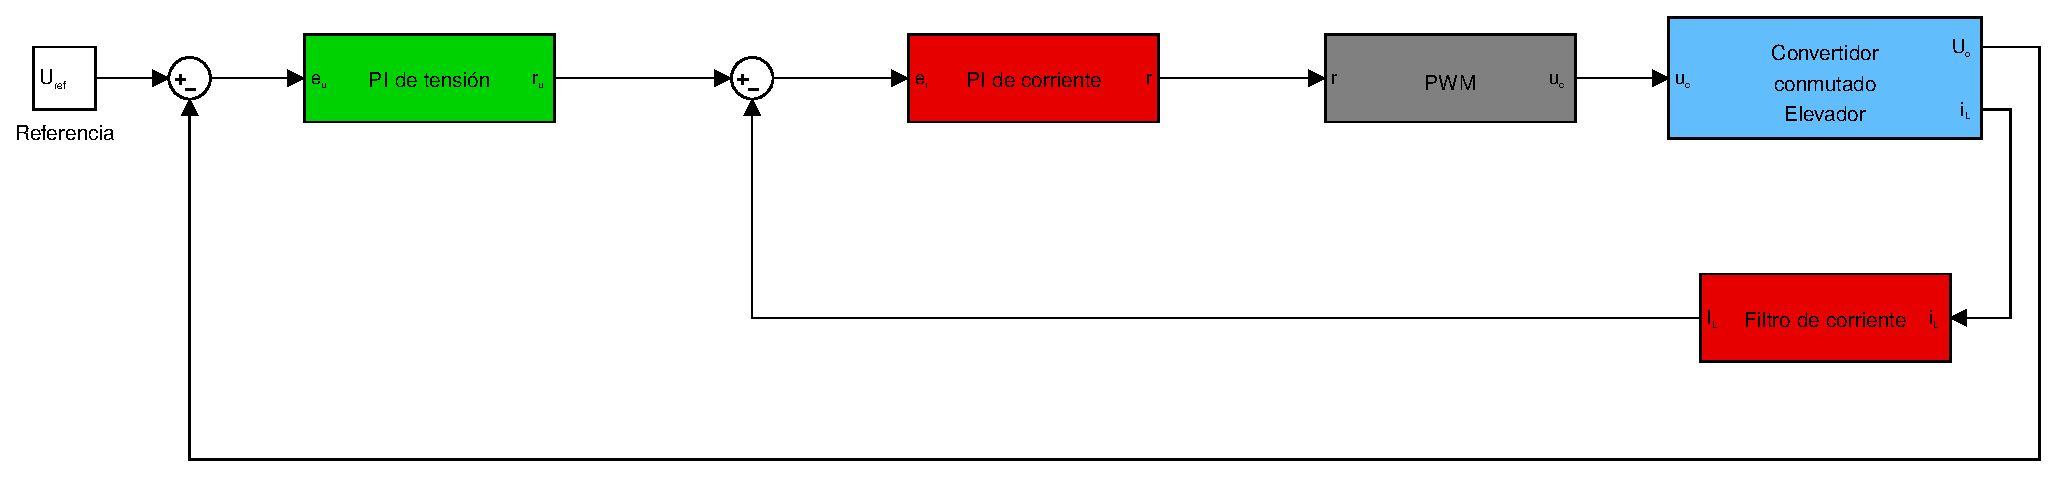
\includegraphics[width=10cm]{gfx/esquema_control_elevador.eps}\label{fig:esquema_control_elevador}} \\
 \subfloat[Esquema de control para el reductor]{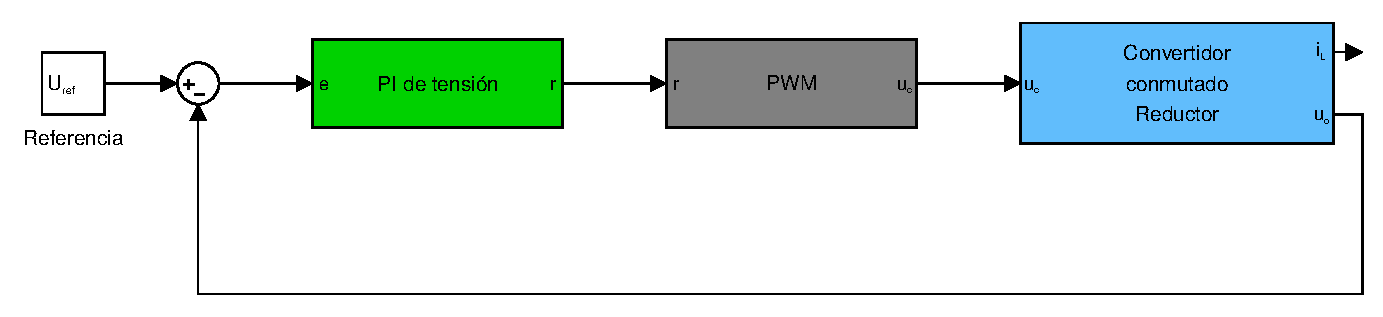
\includegraphics[width=8cm]{gfx/esquema_control_reductor.eps}\label{fig:esquema_control_reductor}}
\end{figure}

Es necesario remarcar la clara diferencia de complejidad que existe entre ambos esquemas. La fig. \ref{fig:esquema_control_elevador} presenta dos lazos de realimentación
mientras que la fig. \ref{fig:esquema_control_reductor} solo presenta uno. Esto se debe al hecho de que la ecuación de de estado que define a la tensión de salida del
elevador es inestable si no se controla la corriente, y es por ello que se decidió colocar un lazo de realimentación interno para controlar la corriente. La presencia
del filtro de realimentación de corriente es importante debido al gran rizado que posee la corriente, asimismo esto permite que las señales utilizadas en los controladores
sean de una naturaleza acorde al diseño propuesto ya que de otro modo la presencia del rizado de corriente anularía las suposiciones hechas al momento de su diseño, en las
que se asumió una reducida variabilidad alrededor de los puntos de trabajo.

Por otro lado, el convertidor reductor es de naturaleza inherentemente estable y no es necesario controlar la corriente para lograr la estabilidad del sistema. Esto permite
la posterior utilización de la medición de corriente en las modificaciones introducidas al control del reductor para realizar el emulador.

Para obtener una sintonía adecuada de los parámetros de los controladores PI, se utilizó la herramienta \emph{sisotool} de MATLAB.

El análisis dinámico que se realizó, fue utilizado con el fin de obtener los parámetros de diseño de los controladores. A continuación se presentan los procedimientos
abordados para el diseño.

\subsection{Sintonía de controladores para elevador}
\label{sub:sintonia_elevador}
A partir de la El filtro de corriente se encargará de eliminar las altas frecuencias debidas a la conmutación del modulador de ancho de pulso, por lo que
debe considerarse una frecuencia de corte suficiente para que el rizado de corriente no afecte la acción de control. Para la sintonía se han dispuesto los
bloques del esquema de la fig. \ref{fig:esquema_control_elevador} según las funciones de transferencia que los caracterizan. Esta representación se encuentra
en la fig. \ref{fig:esquema_control_elevador_lineal}.

\begin{figure}[H]
  \centering
  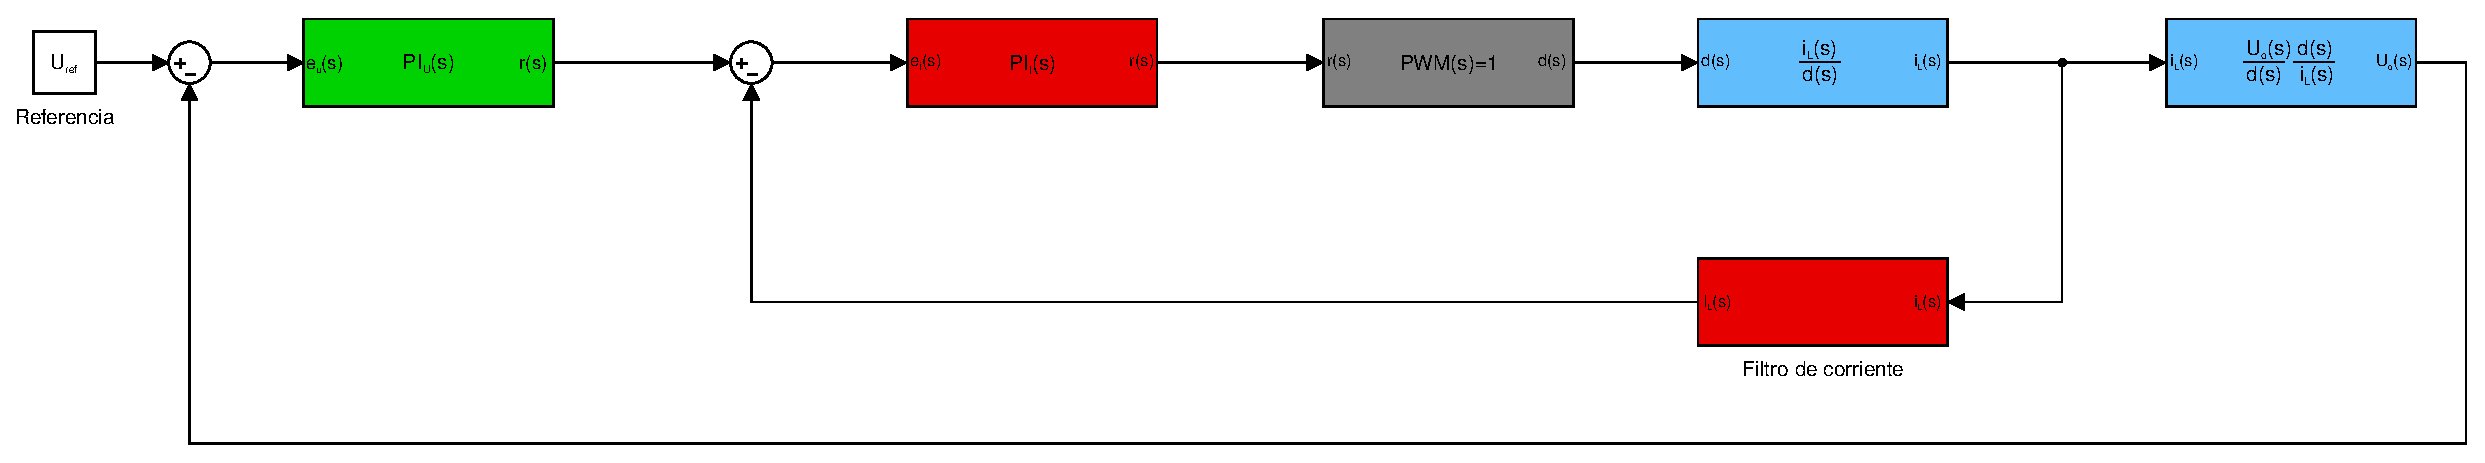
\includegraphics[width=10cm]{gfx/esquema_control_elevador_lineal.eps}
  \caption{Esquema linealizado del control del elevador.}
  \label{fig:esquema_control_elevador_lineal}
\end{figure}

Los controladores fueron diseñados con la estructura típica que los define en el dominio $Z$ según $PI(z)=K_{P}+\frac{T_{s}K_{I}}{z-1}$.
En la figura se muestra el análisis en el lugar de las raíces respecto al lazo de tensión.

\begin{figure}[H]
  \centering
  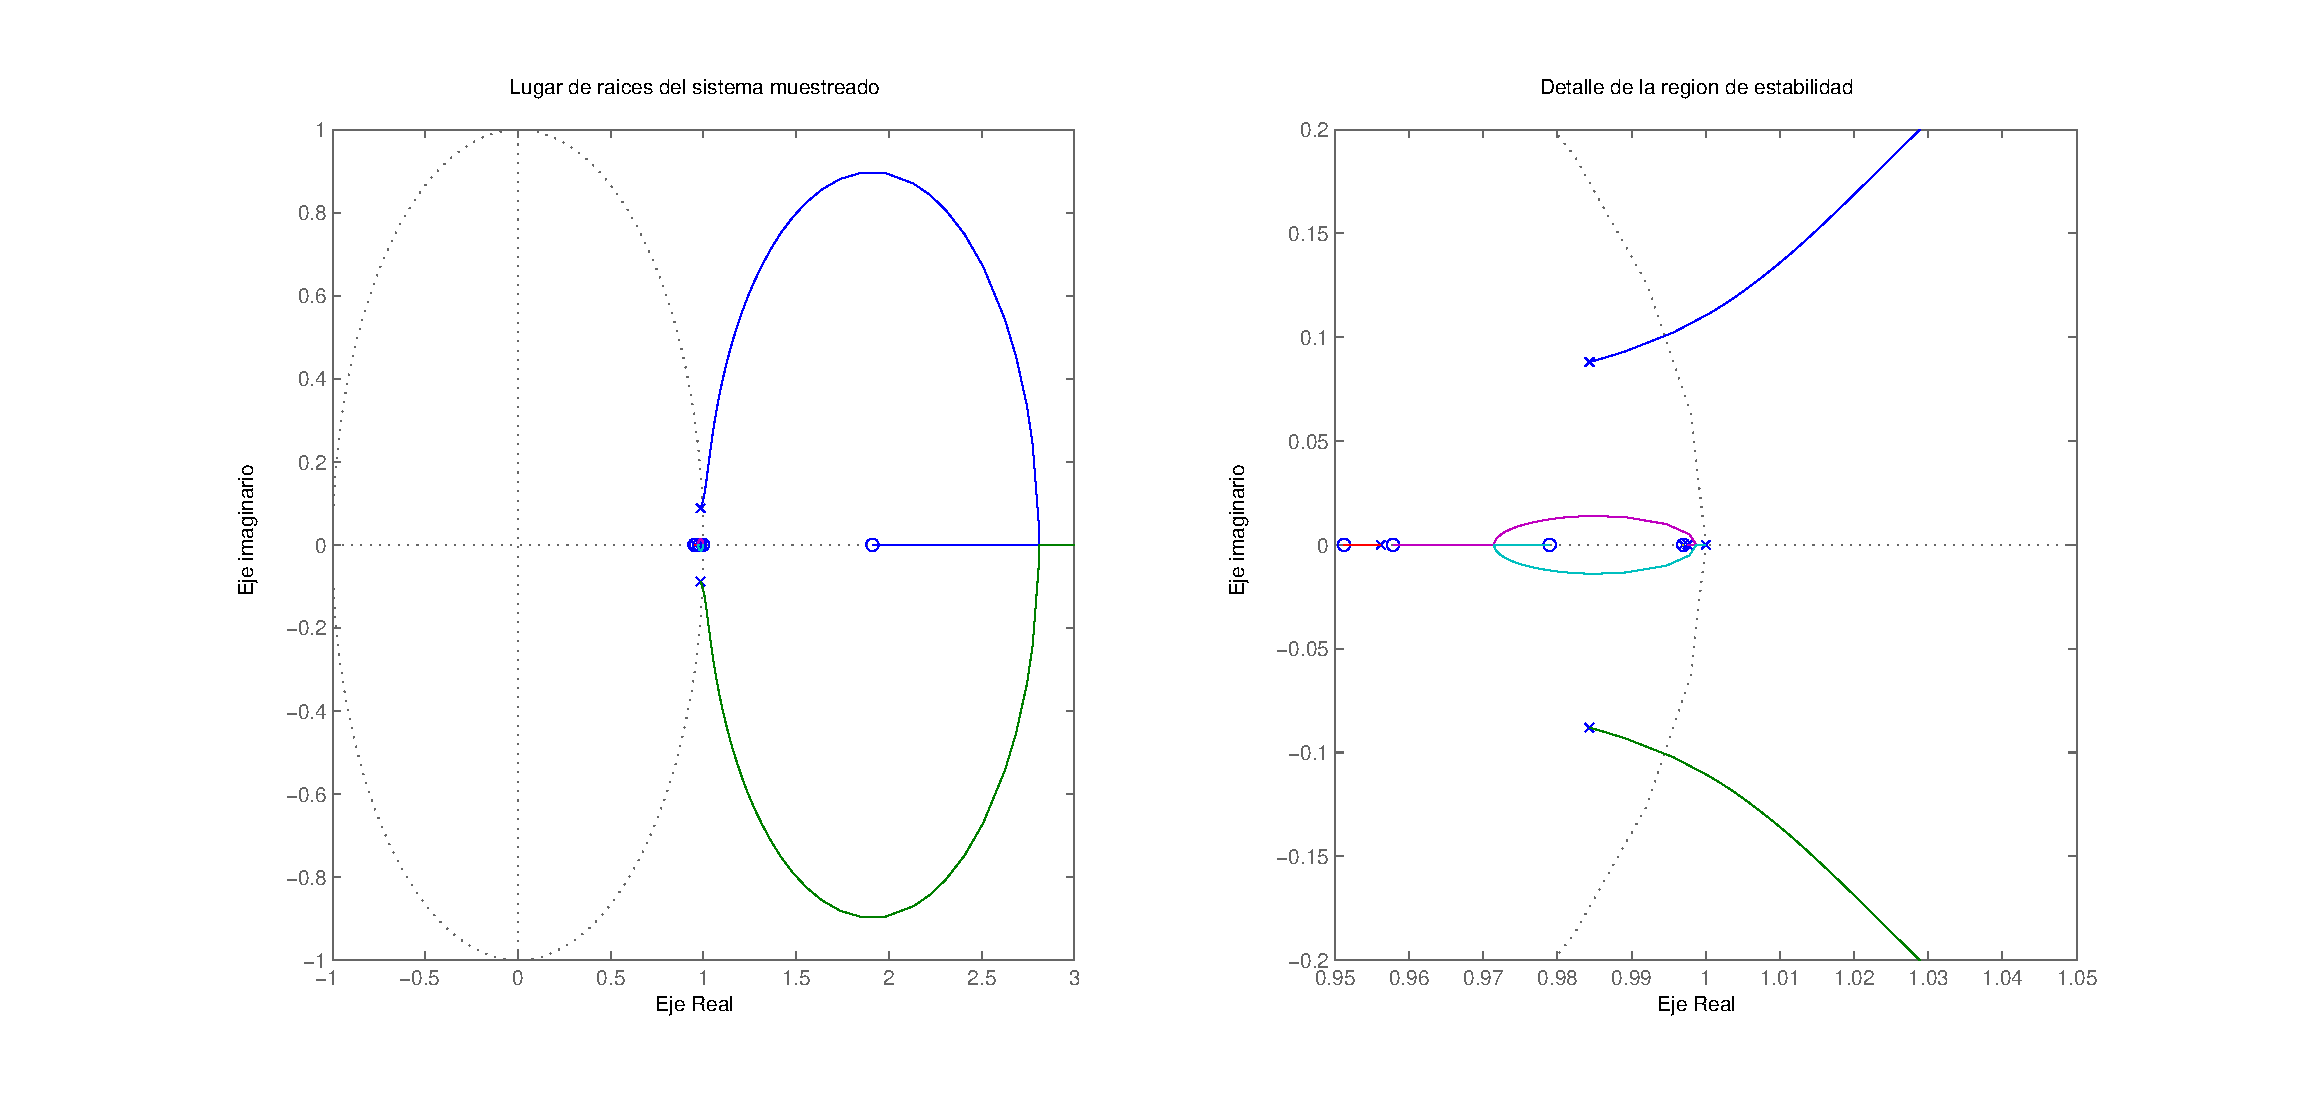
\includegraphics[width=11cm]{gfx/rlocus_elevador.eps}
  \caption{Análisis del lugar de las raíces en el dominio $Z$ para $T_{s}=50\mu s$}
  \label{fig:rlocus_elevador}
\end{figure}

Puede observarse que la región de estabilidad es bastante acotada por lo que para obtener un buen comportamiento del elevador, los parámetros
debieron ser seleccionados con bastante precisión. Los parámetros del controlador de corriente se eligieron partiendo
del \emph{criterio de la respuesta al escalón de Ziegler–Nichols } mientras que para el controlador de corriente se usó el \emph{criterio de la
respuesta en frecuencia de Ziegler–Nichols }.

En la tabla \ref{tab:parametros_control_elevador} se muestran los parámetros obtenidos.

\begin{table}[H]
  \centering
  \begin{tabular}{|c|c|c|}
    \hline 
    Controlador 	& $K_{P}$ 	& $K_{I}$	\tabularnewline \hline \hline 
    PI corriente 	& 0.03 		& 7		\tabularnewline \hline 
    PI tensión 		& 0.16 		& 150		\tabularnewline \hline 
    \end{tabular}
    \caption{Parámetros del controlador del elevador.}
    \label{tab:parametros_control_elevador}
\end{table}

\subsection{Sintonía de controlador para reductor}
Dada la simplicidad del sistema en este caso se implementará un esquema de control simple para obtener la tensión buscada utilizando un controlador
PI en el que se medirá la tensión y se buscará ajustar la misma para seguir de un valor de referencia , por lo que será más sencillo diseñar
el controlador. Este diseño puede ser encarado de esta manera, debido a que no existen los problemas de estabilidad que se tenían en el
elevador. Por lo tanto, para esta etapa no será necesario el sensado de la corriente, aunque esta información será utilizada en una etapa
posterior del desarrollo del proyecto. El esquema puede verse en la fig. \ref{fig:esquema_control_reductor_lineal}.

\begin{figure}[H]
  \centering
  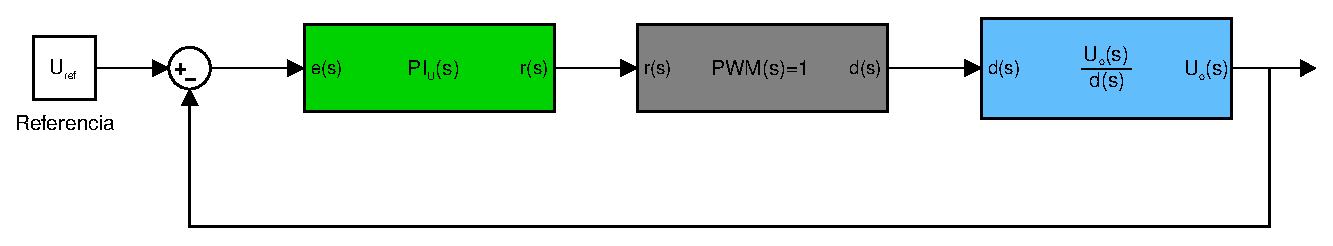
\includegraphics[width=10cm]{gfx/esquema_control_reductor_lineal.eps}
  \caption{Esquema de control del Reductor.}
  \label{fig:esquema_control_reductor_lineal}
\end{figure}

El diagrama de lugar de raíces del sistema muestreado puede verse
en la fig. \ref{fig:rlocus_reductor}.

\begin{figure}[H]
  \centering
  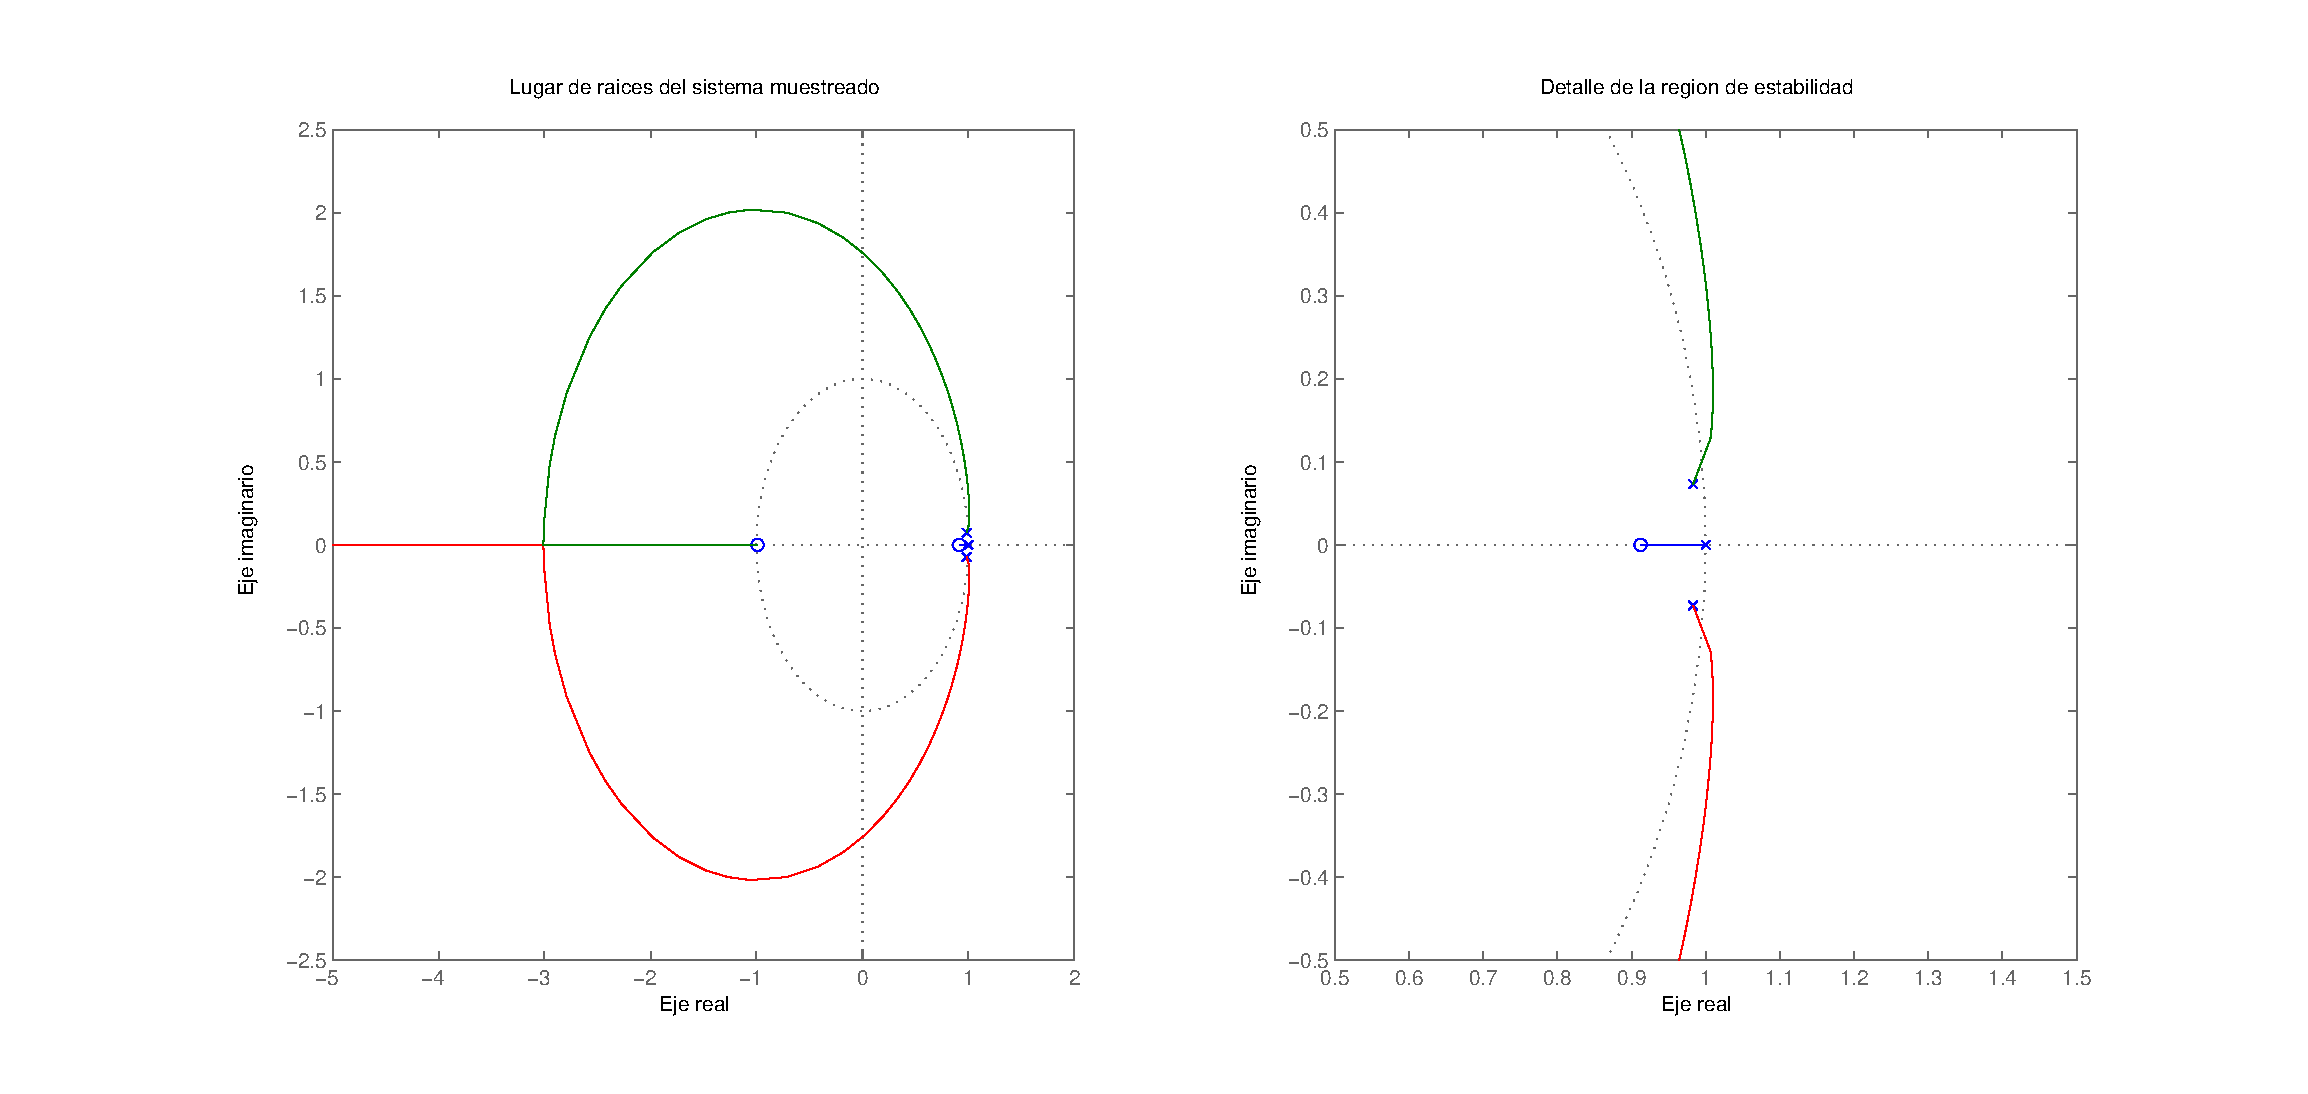
\includegraphics[width=11cm]{gfx/rlocus_reductor.eps}
  \caption{Diagrama del lugar de raíces para el lazo de tensión del reductor.}
  \label{fig:rlocus_reductor}
\end{figure}

En el cuadro \ref{tab:parametros_control_reductor} se listan los parámetros obtenidos.

\begin{table}[H]
  \centering
  \begin{tabular}{|c|c|c|}
    \hline 
    Controlador 	& $K_{P}$ 	& $K_{I}$\tabularnewline \hline \hline 
    PI tensión 		& 0.05 		& 10\tabularnewline \hline 
  \end{tabular}\caption{Parámetros del controlador del reductor}
  \label{tab:parametros_control_reductor}
\end{table}

\section{Modelos y simulaciones}
Ya definidos los controladores y los modelos de estados de cada convertidor, se procedió a la utilización de los programas de cómputo para realizar
simulaciones que sirvan de prueba preliminar previas a la puesta en marcha del equipo. Estos resultados se muestran en las siguientes secciones.
Cabe aclarar que la fuente de potencia utilizada para alimentar los convertidores posee una limitación de corriente de 18A máximos y ello se verá
en las curvas de funcionamiento presentadas. Las simulaciones comprenden las mediciones de corriente y tensión ante la puesta en marcha de los convertidores
y una perturbación en la carga aplicada.
\subsection{Convertidor elevador}
El modelo utilizado puede verse en la figura \ref{fig:modelo_elevador} en el que se distingue el esquema físico en la parte superior del hardware
de control en la parte inferior, compuesto por el conversor analógico-digital, el controlador y el generador PWM.

\begin{figure}[H]
  \centering
  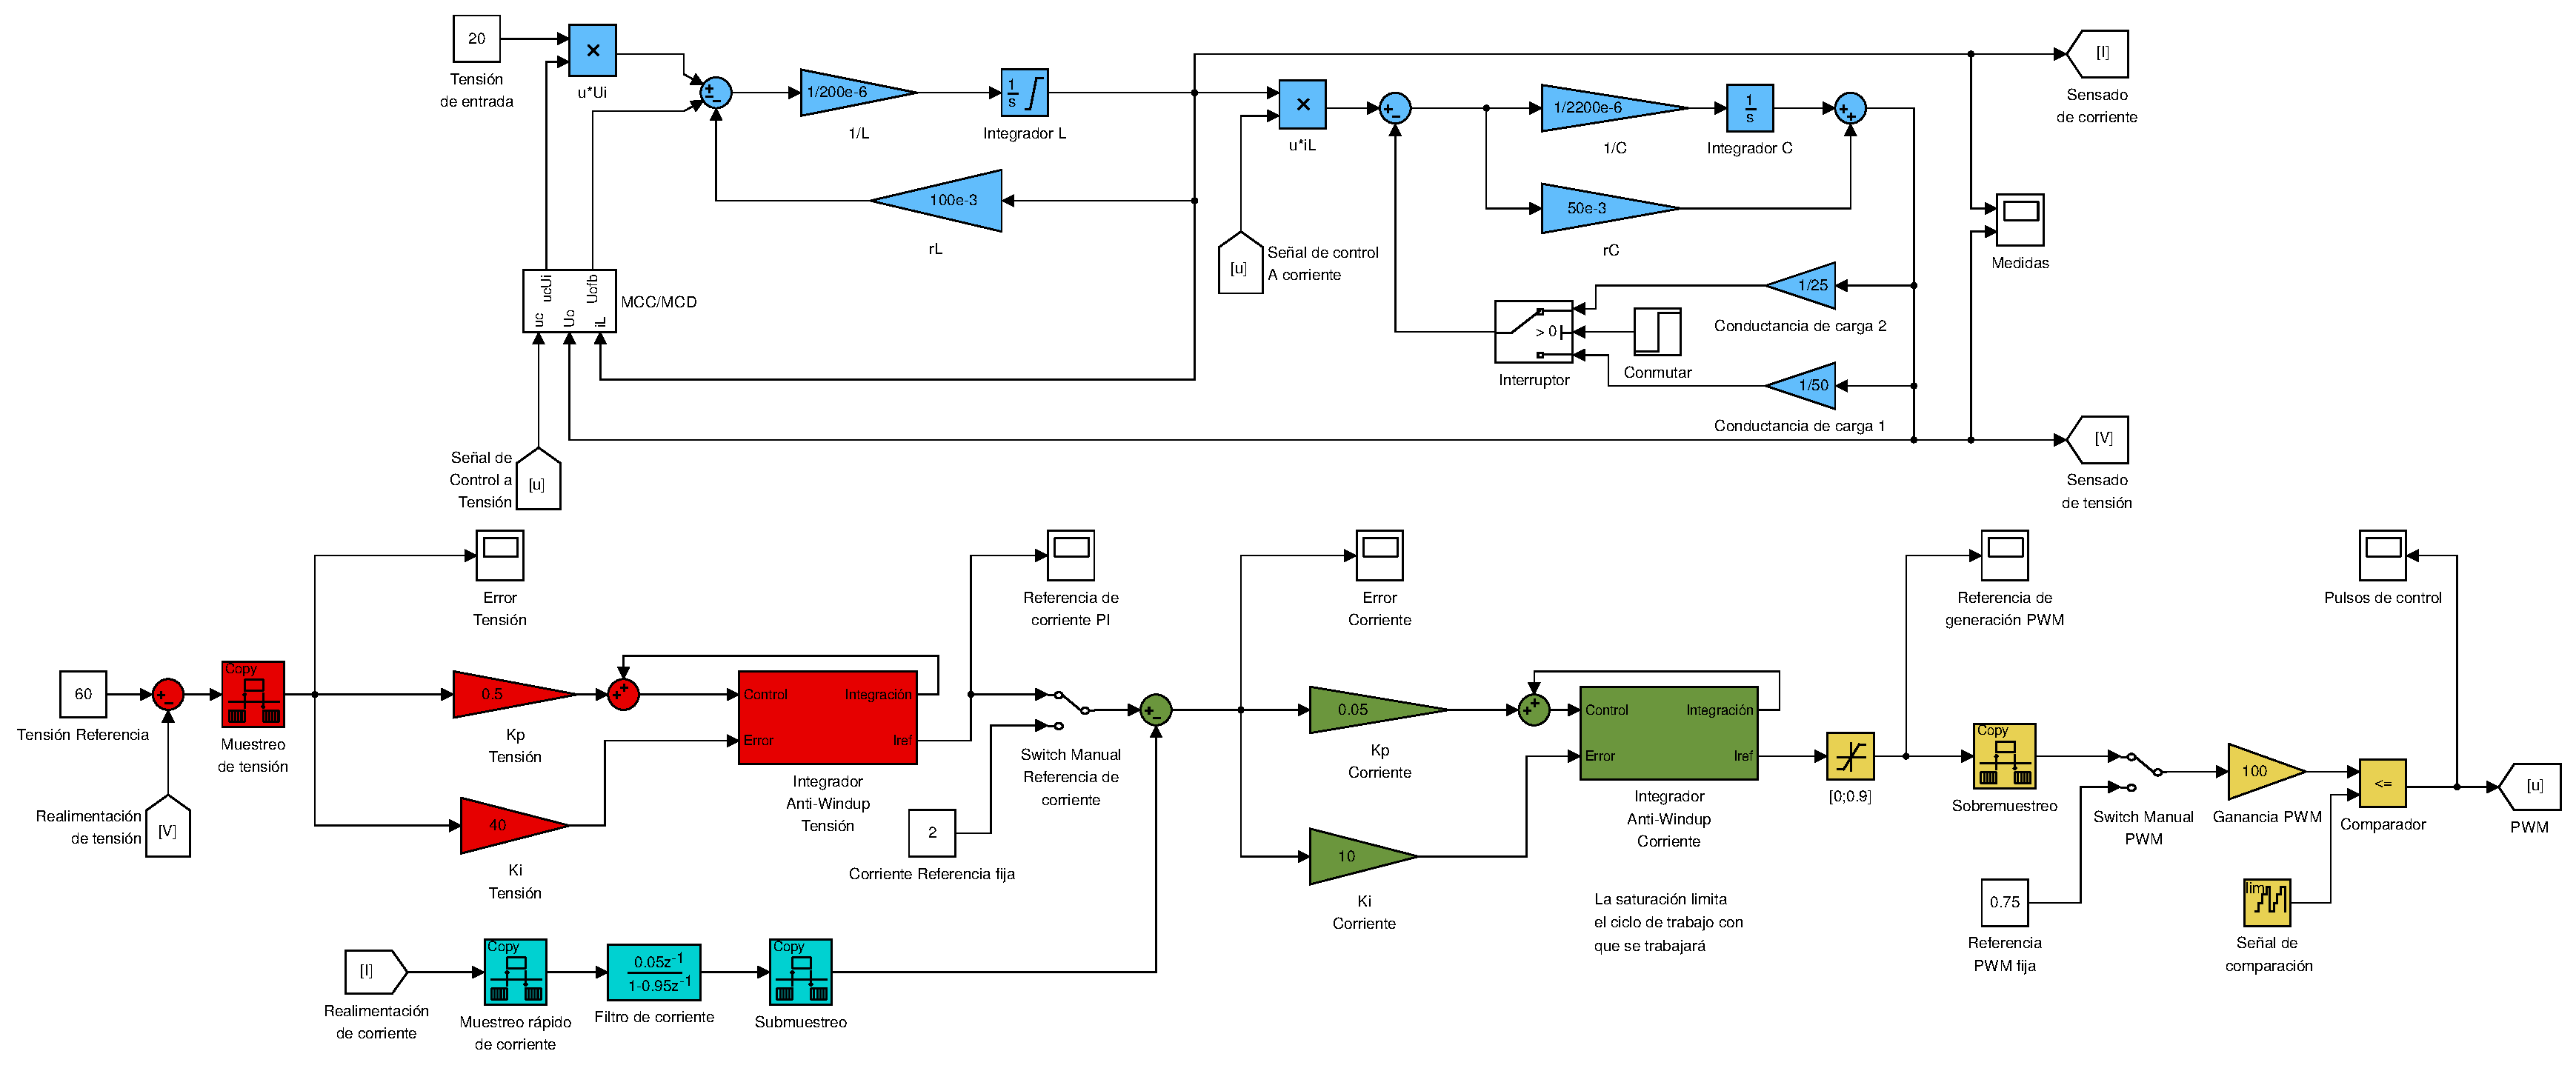
\includegraphics[width=11cm]{gfx/modelo_elevador.eps}
  \caption{Modelo completo del convertidor elevador}
  \label{fig:modelo_elevador}
\end{figure}


La figura \ref{fig:curvas_elevador} muestra el resultado de simulación del encendido del convertidor elevador con una tensión inicial de
capacitor igual a la tensión de entrada. La corriente del inductor ha sido limitada a 15 A como puede verse en la imagen.

\begin{figure}[H]
  \centering
  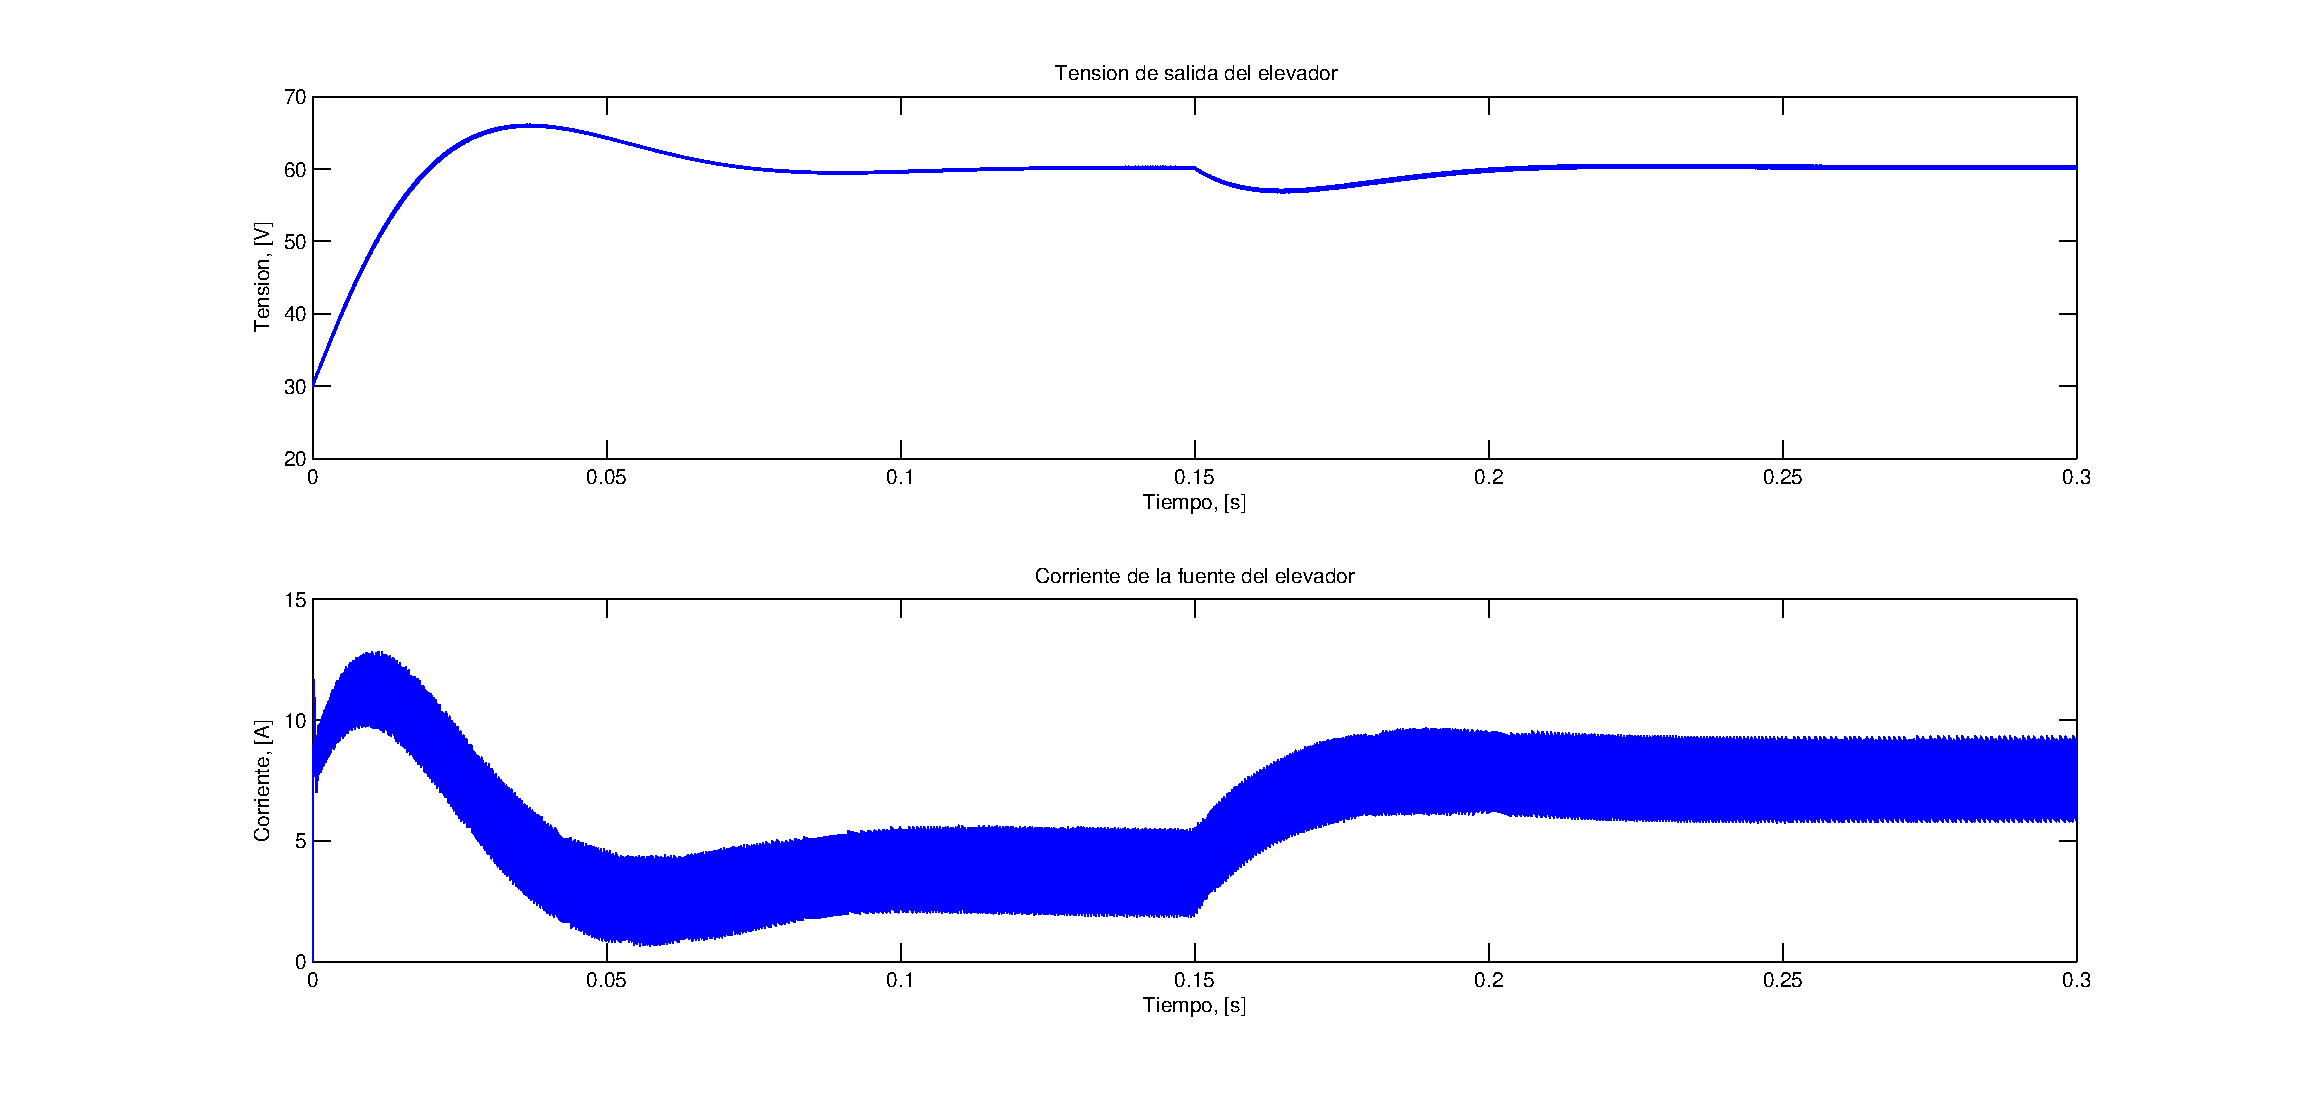
\includegraphics[width=11cm]{gfx/curvas_elevador.eps}
  \caption{Resultado de simulación de corriente de inductor y tensión de salida del convertidor DC-DC elevador}
  \label{fig:curvas_elevador}
\end{figure}

\subsection{Convertidor reductor}
El modelo de simulación del reductor puede verse en la figura \ref{fig:modelo_reductor}. El modelo físico del hardware se encuentra en la parte
superior y el sistema de control en la parte inferior.

\begin{figure}[H]
  \centering
  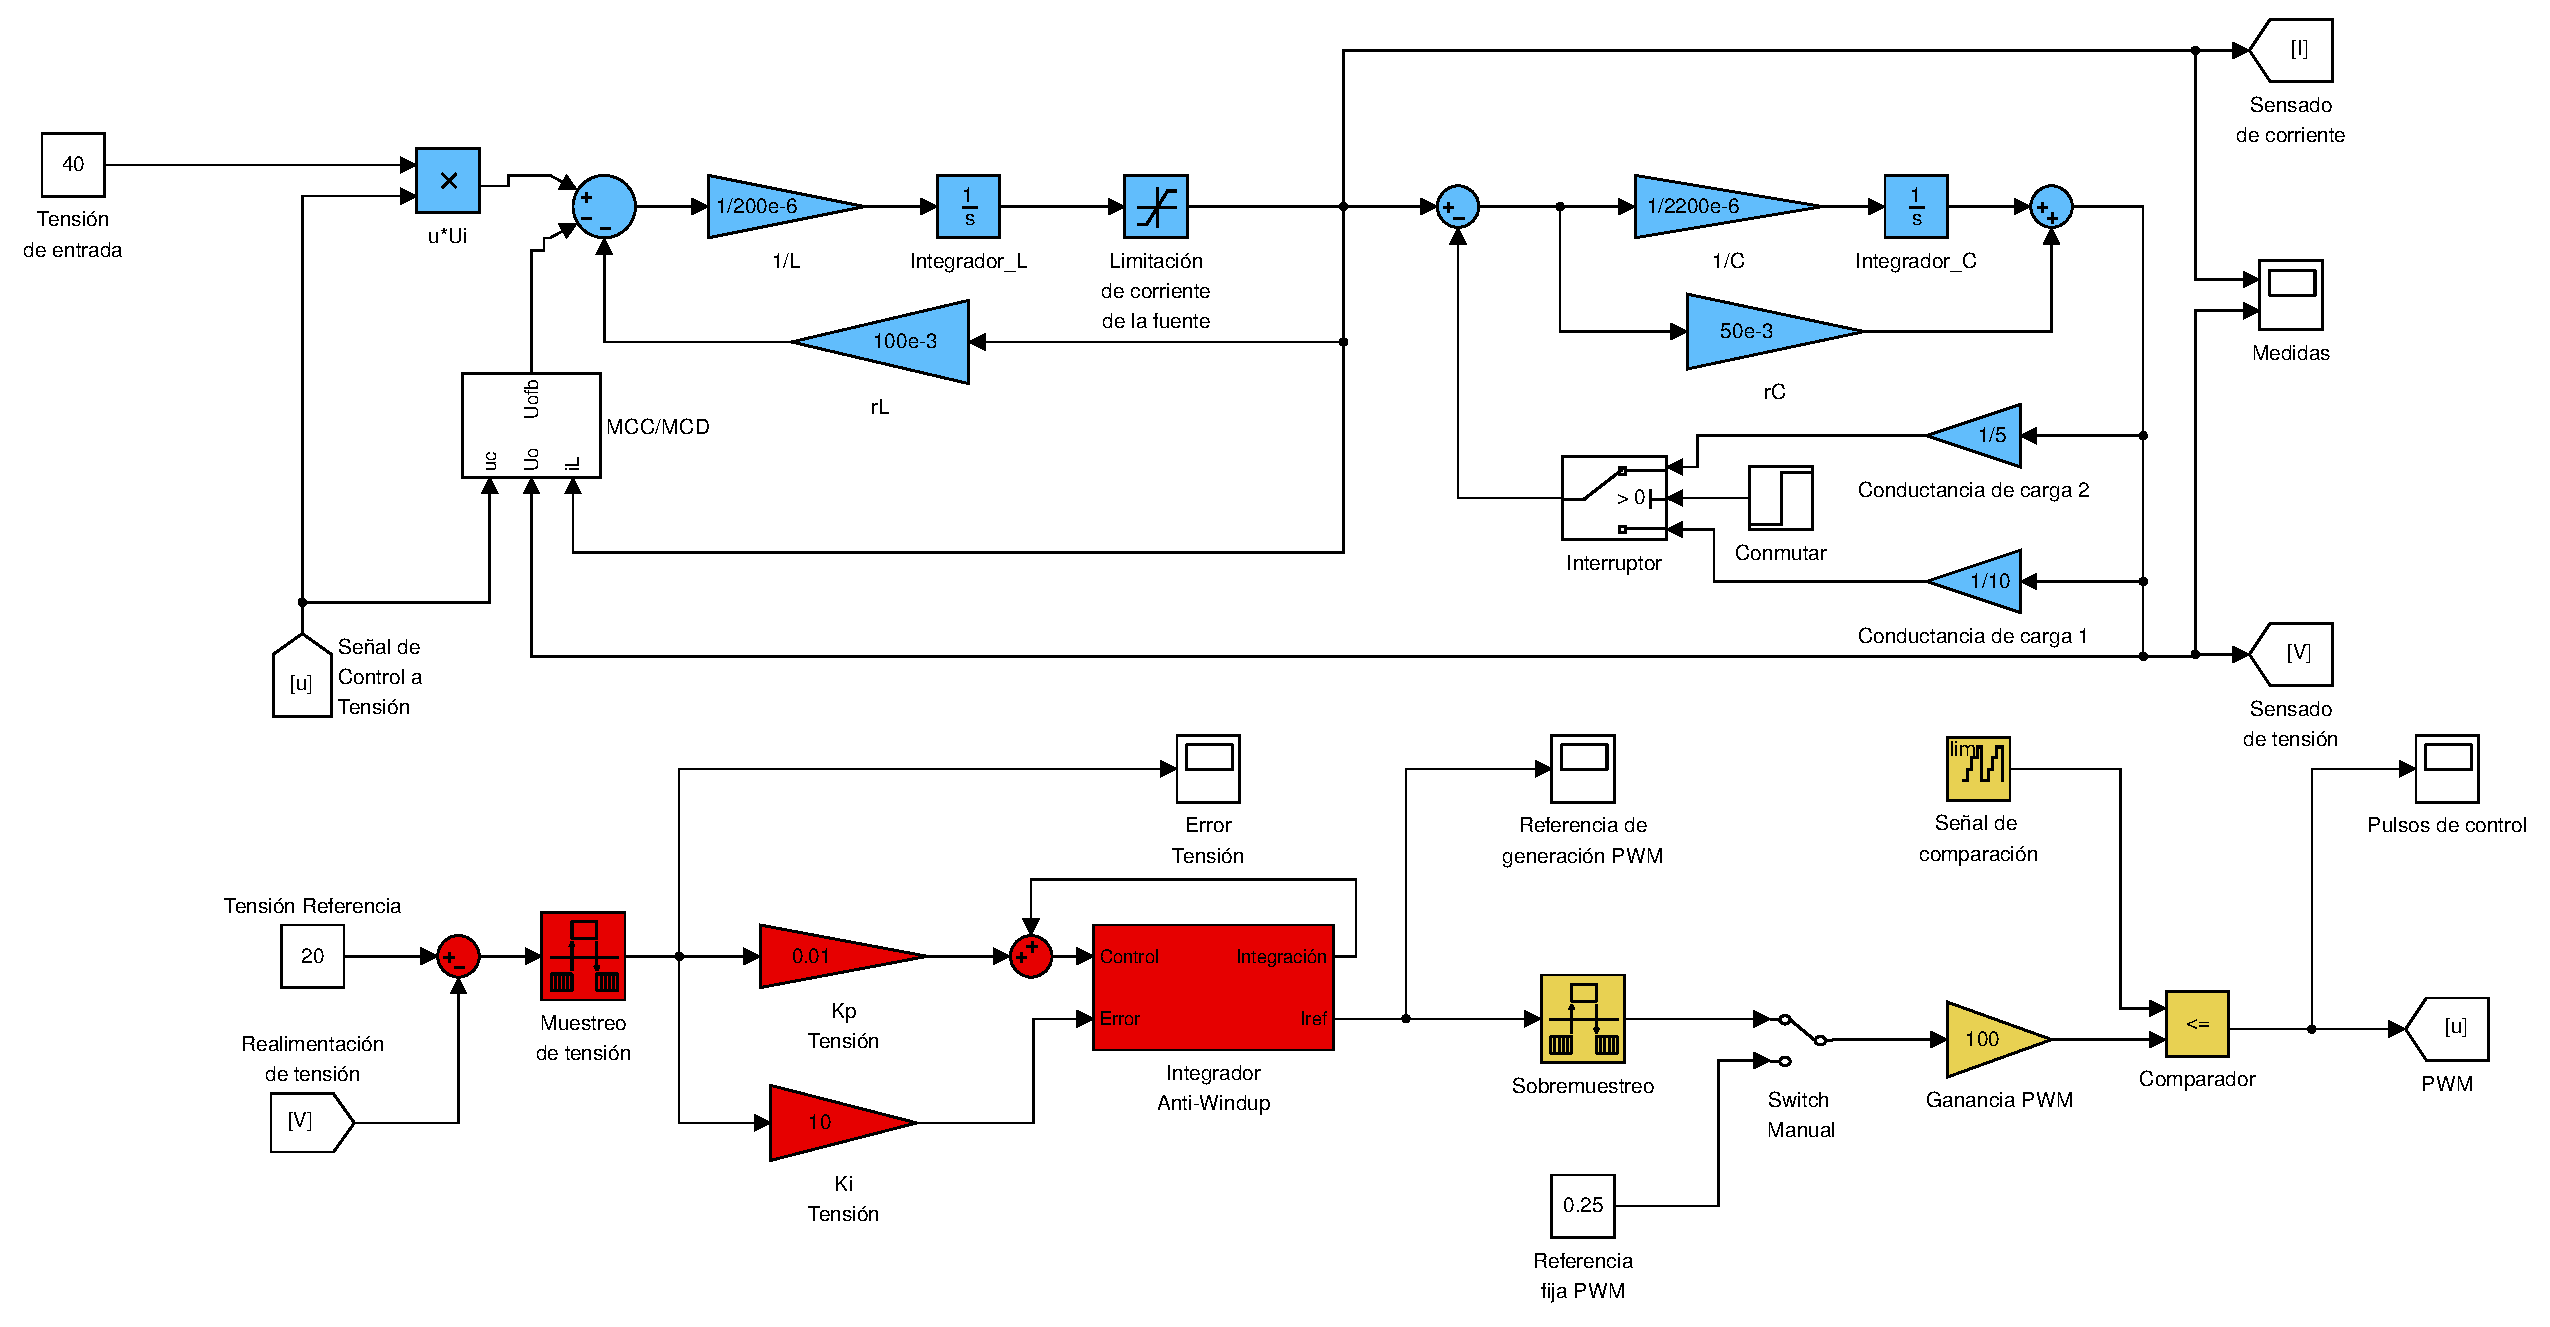
\includegraphics[width=11cm]{gfx/modelo_reductor.eps}
  \caption{Modelo completo del convertidor reductor}
  \label{fig:modelo_reductor}
\end{figure}
En la figura \ref{fig:curvas_reductor} puede verse el resultado de la simulación del encendido del convertidor reductor con condiciones
iniciales nulas de tensión y corriente. Puede verse que la corriente también ha sido limitada a 15A para establecer un margen de seguridad.
\begin{figure}[H]
  \centering
  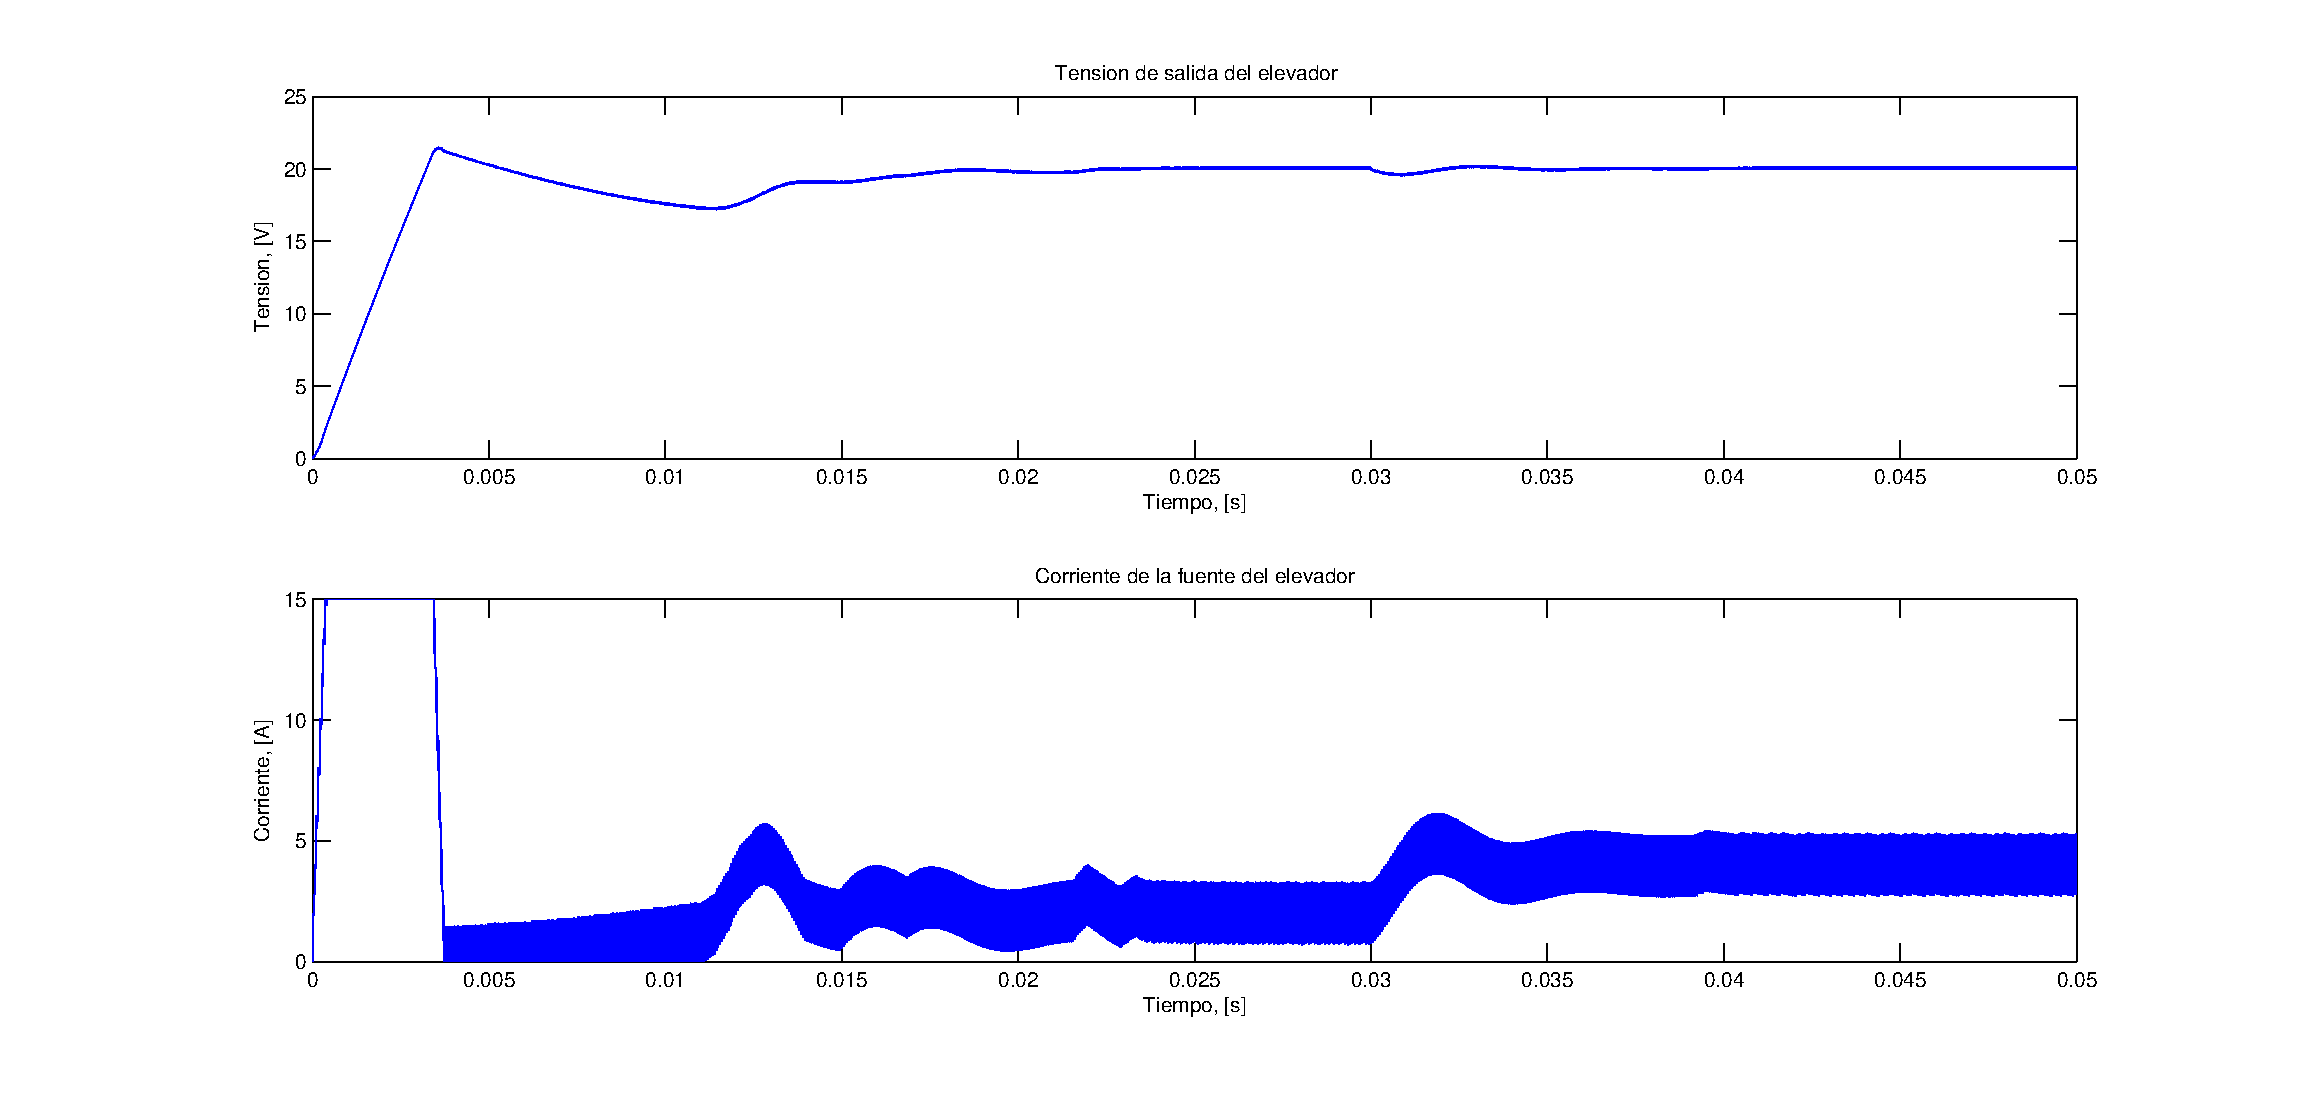
\includegraphics[width=11cm]{gfx/curvas_reductor.eps}
  \caption{Resultado de simulación de corriente de inductor y tensión de salida del convertidor DC-DC reductor}
  \label{fig:curvas_reductor}
\end{figure}

\subsection{Simulación de la operación conjunta de convertidores}

El emulador propuesto en el proyecto fue pensado para poder ser acoplado a un sistema híbrido de generación de energía y es conectado a éste
a través de un sistema de potencia que se trata del convertidor DC-DC elevador que se ha estudiado. Por lo tanto para proceder ordenadamente 
en la unificación de los proyectos se propuso el ensayo de la interconexión de los convertidores para poder realizar pruebas de la parte
del SGH  que comprende la pila de combustible. Para esto se requirió que el convertidor reductor pueda ser usado para alimentar al convertidor elevador. Por
ello, se dispuso la realización de las simulaciones que estudien el comportamiento de los convertidores acoplados a fin de conocer si
es posible realizar la conexión mencionada. La fig. \ref{fig:modelo_acoplado} muestra el modelo de los dos convertidores acoplados.
\begin{figure}[H]
  \centering
  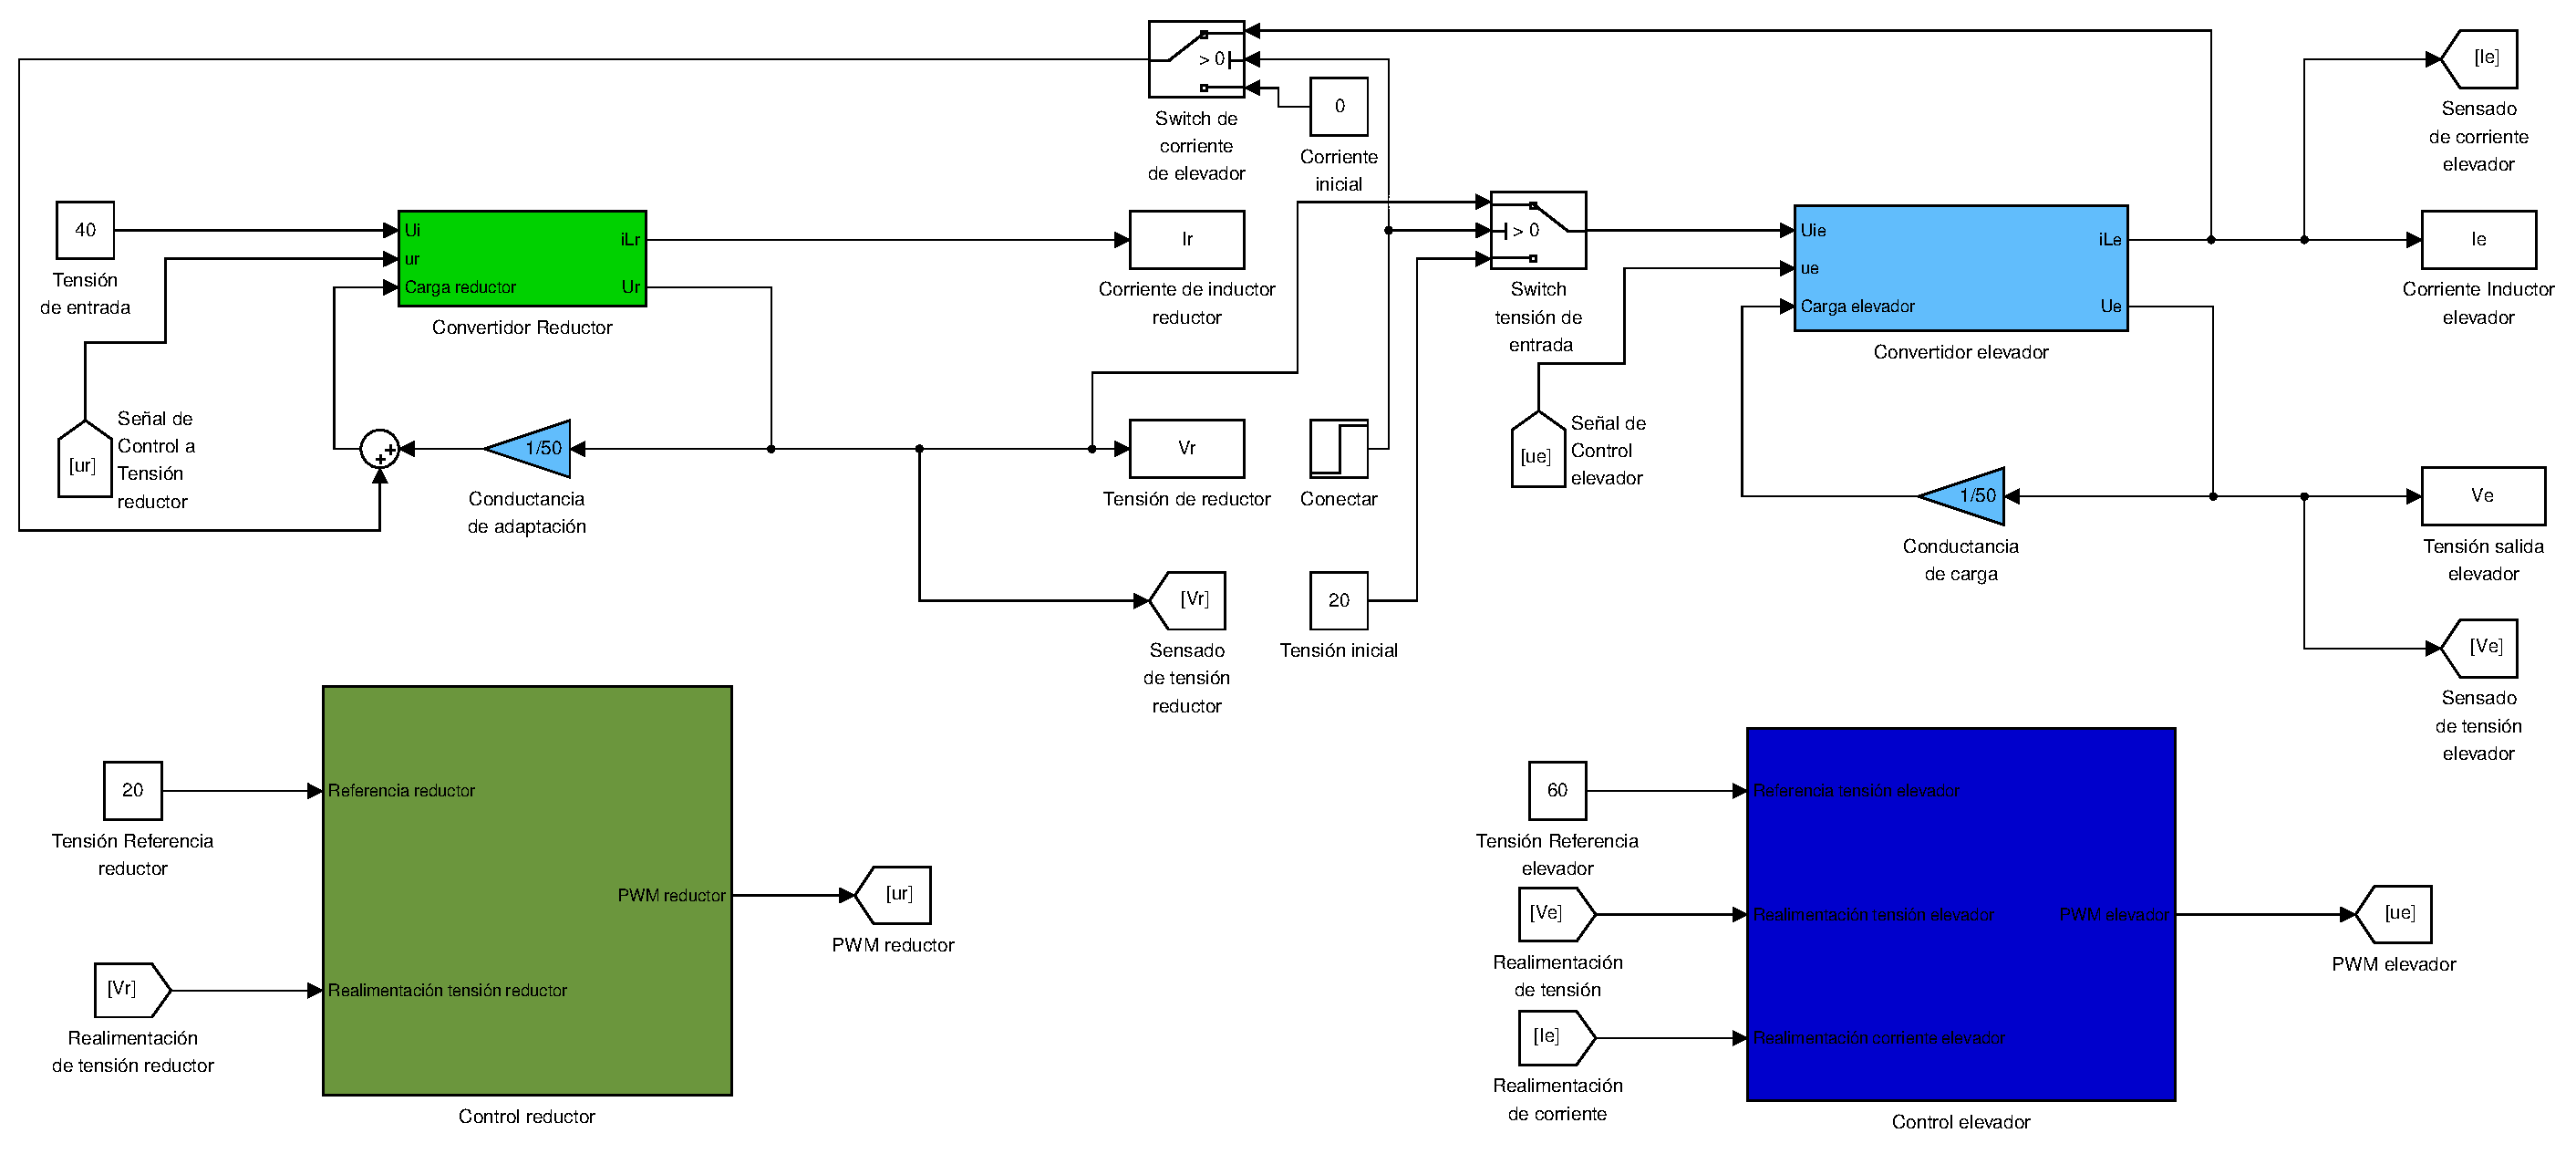
\includegraphics[width=11cm]{gfx/modelo_acoplado.eps}
  \caption{Modelo usado para la simulación del comportamiento conjunto de los convertidores}
  \label{fig:modelo_acoplado}
\end{figure}
En el modelo puede apreciarse que la interconexión se efectúa cuando ambos convertidores alcanzan un régimen permanente operando de forma
aislada, tras lo cual un conmutador realiza la conexión. Los resultados de de la simulación tanto de las medidas de tensión y corriente para
el convertidor reductor y elevador pueden verse en las figuras \ref{fig:reductor_acoplado} y \ref{fig:elevador_acoplado} respectivamente.
\begin{figure}[H]
  \centering
  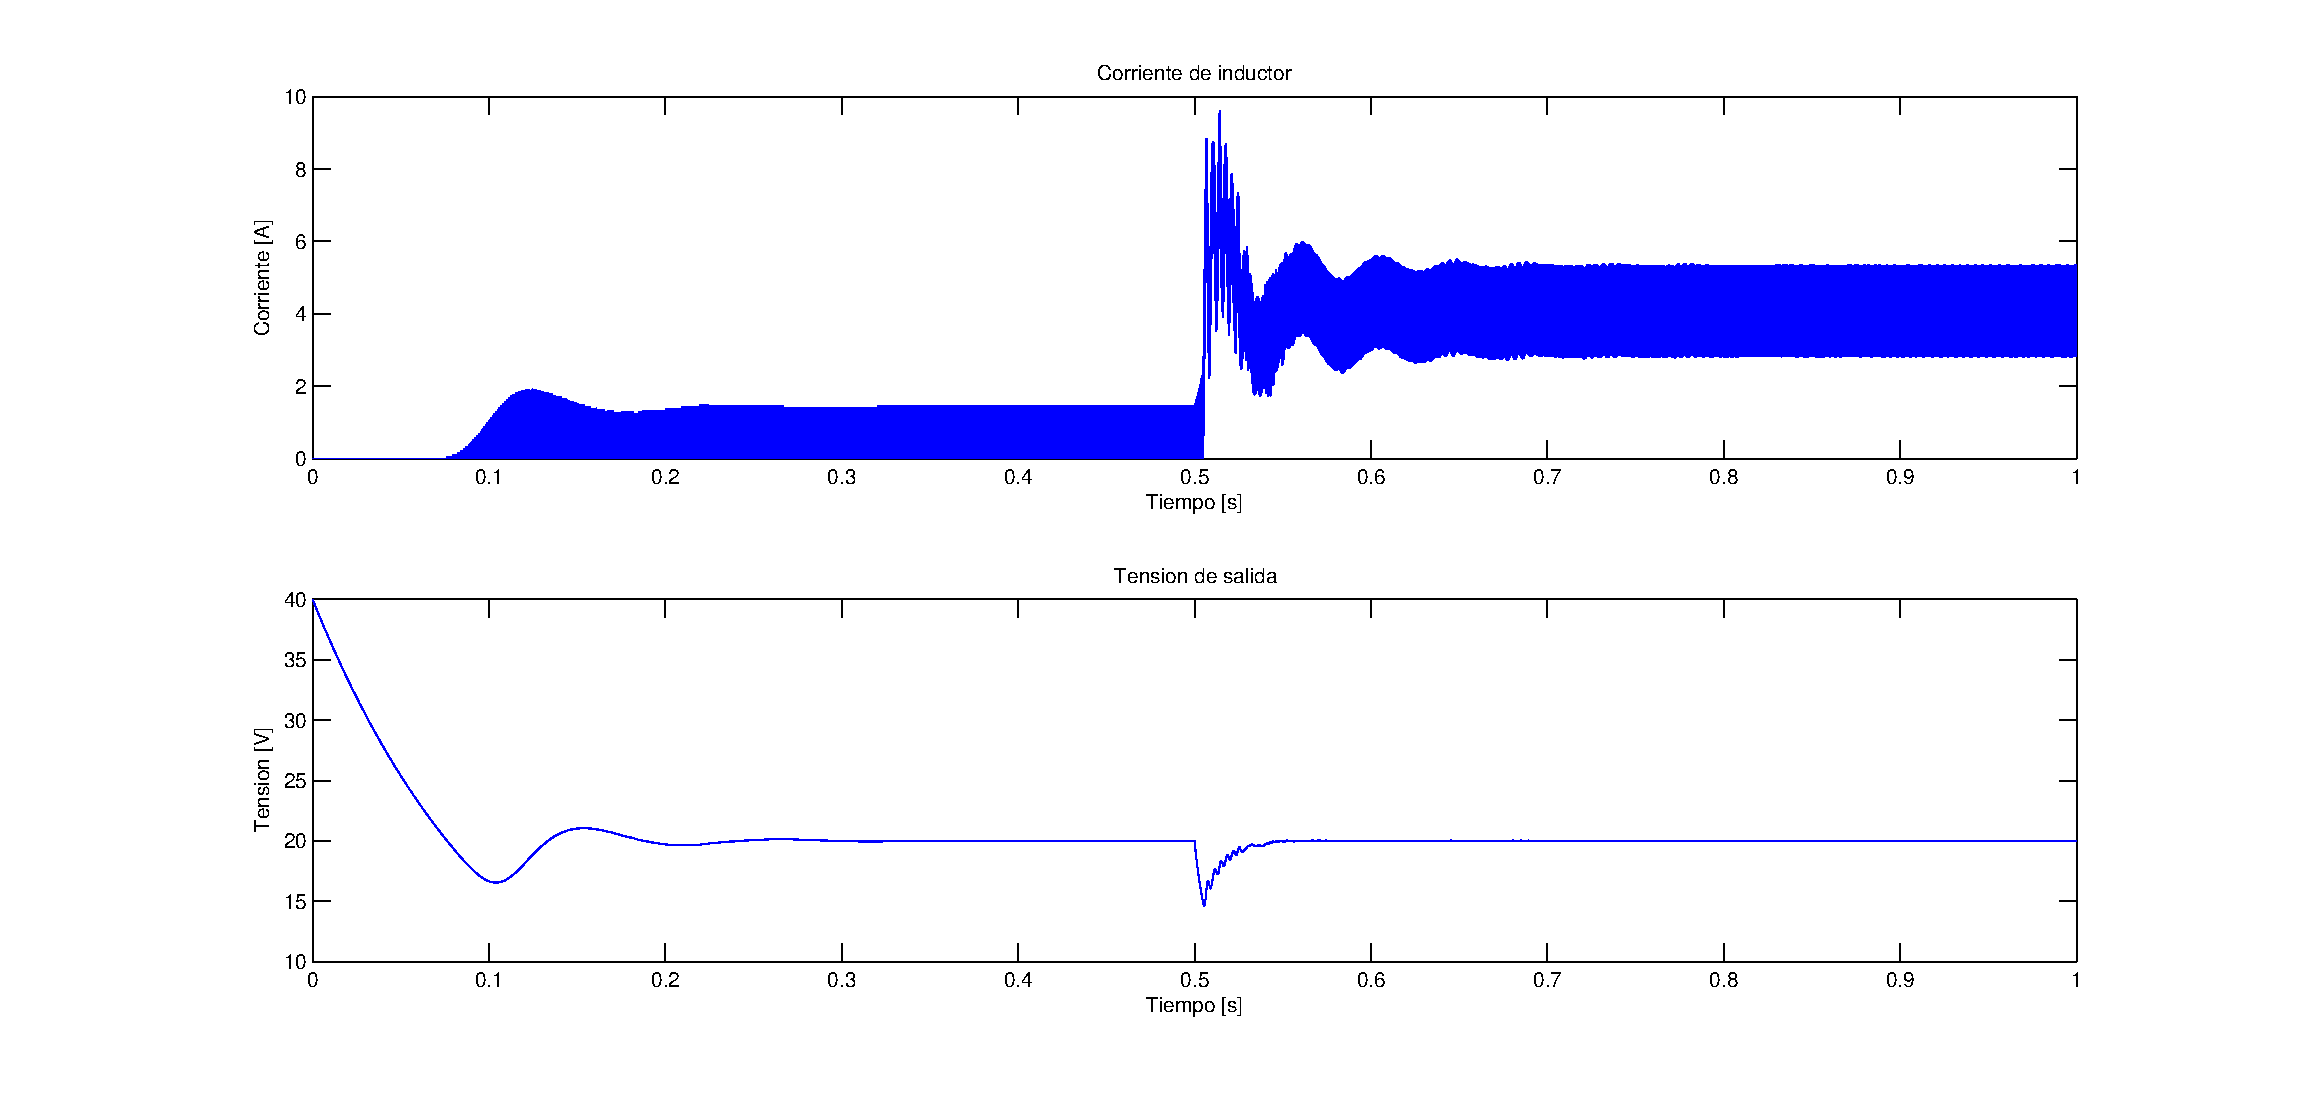
\includegraphics[width=11cm]{gfx/reductor_acoplado}
  \caption{Resultados de la simulación para el convertidor reductor alimentando al elevador}
  \label{fig:reductor_acoplado}
\end{figure}


\begin{figure}[H]
  \centering
  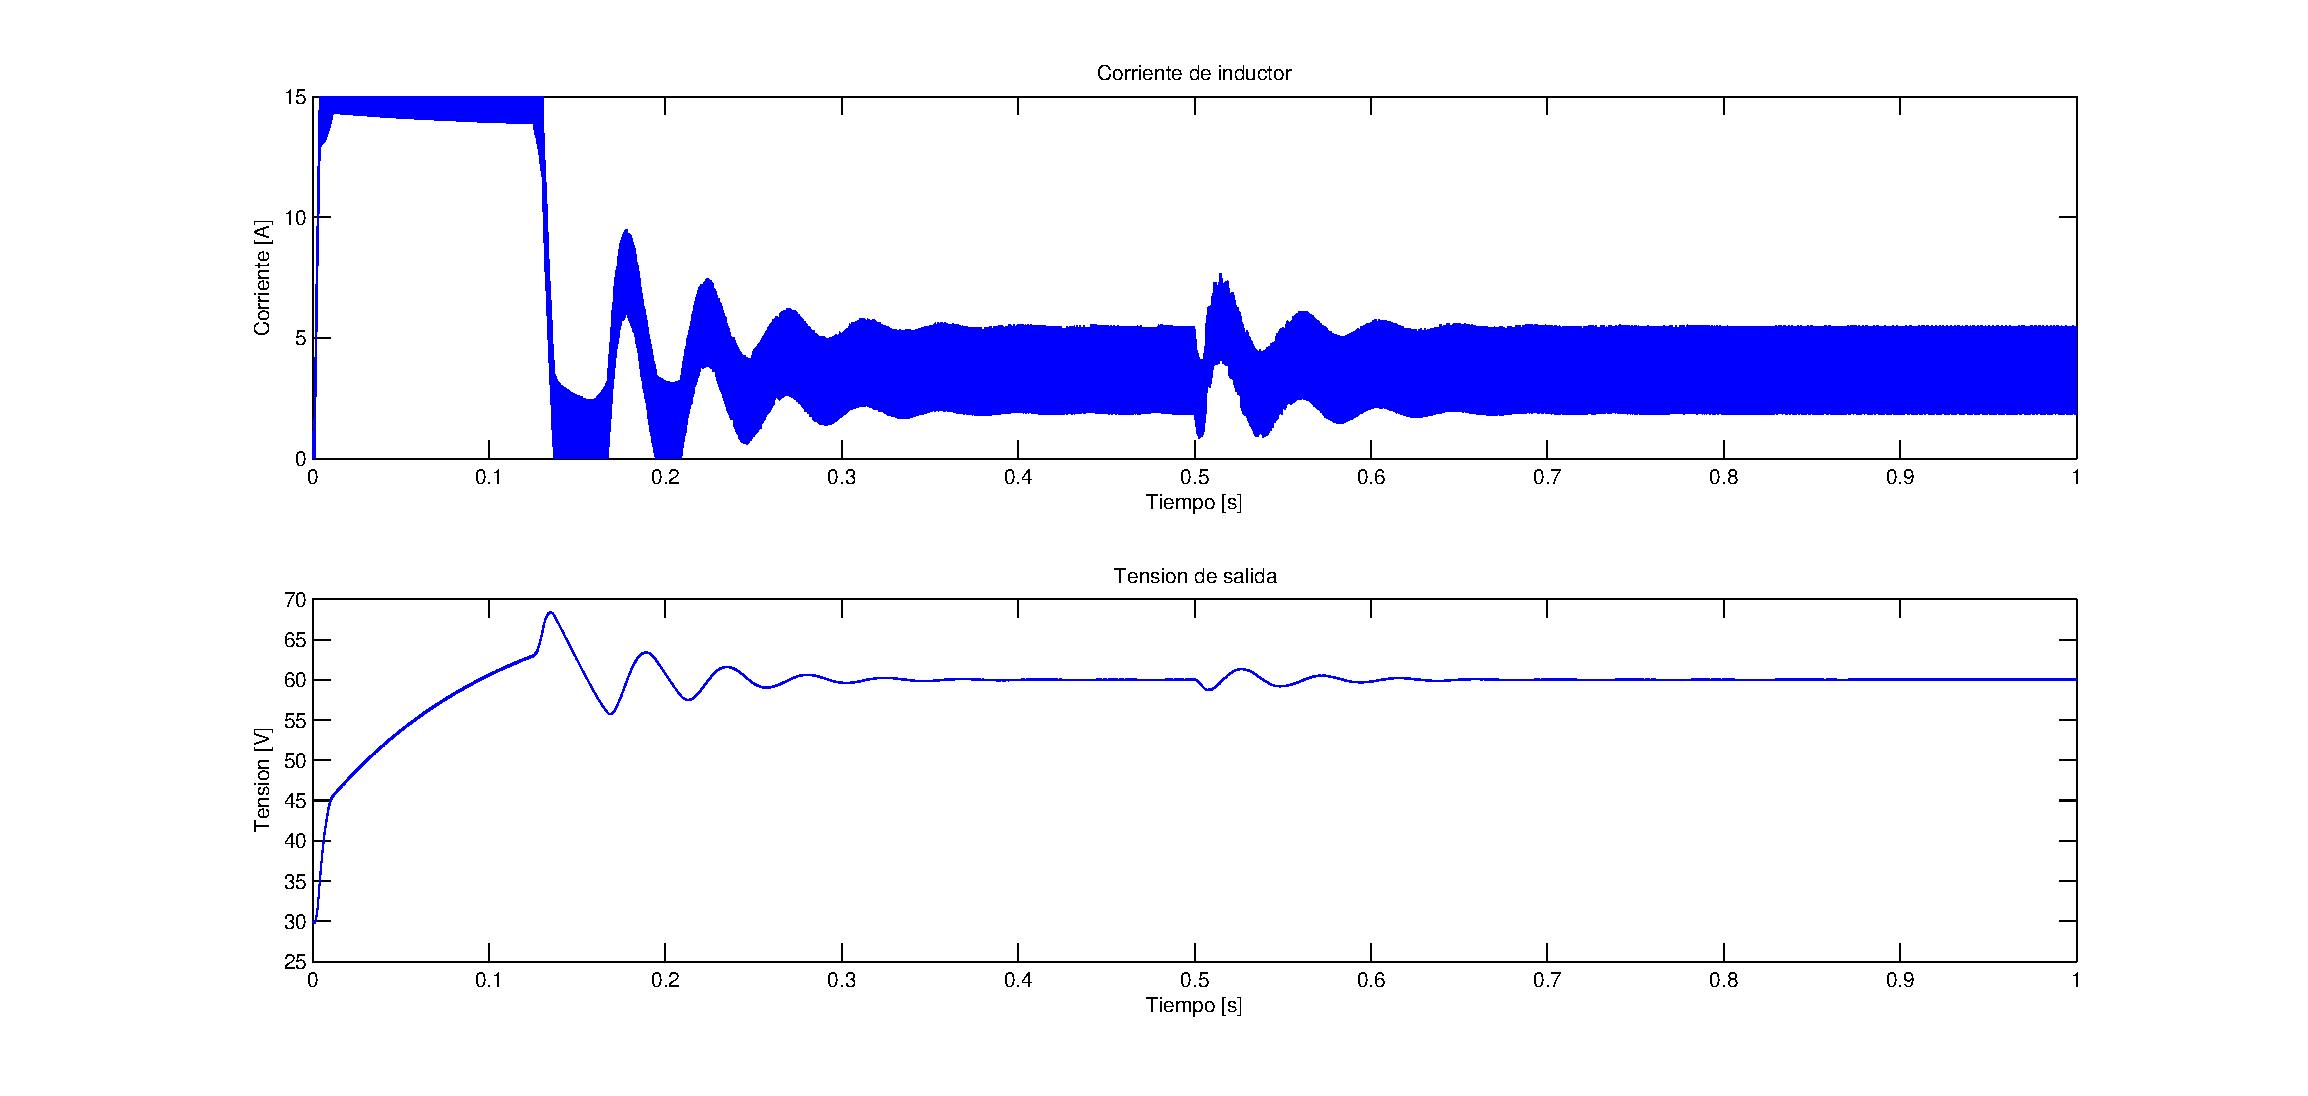
\includegraphics[width=11cm]{gfx/elevador_acoplado}
  \caption{Resultados de simulación para el convertidor elevador alimentado por el reductor}
  \label{fig:elevador_acoplado}
\end{figure}
El conmutador que controla la conexión entre los convertidores se activa al cabo de 0,5s luego del encendido de los convertidores. Los resultados
exhiben un comportamiento adecuado, considerando que los valores devueltos son estables y los convertidores se comportan de acuerdo a lo esperado, 
ya que el convertidor elevador recupera rápidamente los niveles en los que se encontraba mientras que el reductor aumenta el nivel de corriente 
entregada para poder alimentar al convertidor elevador.
\section{Soporte de hardware}
Para la implementación del control se requirió de un dispositivo digital sobre el cual programar los algoritmos diseñados. Con base en el
proyecto del convertidor elevador, se utilizó el mismo \emph{hardware} que el usado para el proyecto del elevador ya que su potencia de cómputo
era suficiente para ejecutar las rutinas programadas y ya se tienen resultados concretos de su correcta funcionalidad para trabajos de esta naturaleza.

El dispositivo utilizado consta de un controlador digital de señales (DSC) recomendado para aplicaciones de electrónica de potencia. Este dispositivo
consta básicamente de una unidad de procesamiento y módulos periféricos cuyas funciones son las de adquisición de señales físicas y presentación de la información.
El módulo de procesamiento trata de un procesador digital de señales, cuya arquitectura esta pensada para la realización de operaciones complejas,
cálculos a gran velocidad y ejecución de rutinas en paralelo. Los módulos periféricos disponibles constituyen entradas y salidas de propósito general(GPIO),
conversores analógico-digitales(ADC) de alta resolución, módulos de comunicación y salidas PWM.

Para el proyecto se utilizaron los módulos de ADC,GPIO y PWM. El módulo ADC fue utilizado para muestrear las medidas tomadas por los circuitos de acondicionamiento, 
el GPIO se ocupó para señales de habilitación y por último el PWM proporcionó las señales de control de las los transistores de conmutación.

Dentro de las características técnicas de mayor interés para el desarrollo del trabajo se cuentan las siguientes:
\begin{itemize}
 \item Frecuencia de la unidad central de procesamiento: 150MHz.
 \item Unidad de punto flotante.
 \item Longitud de los registros: 32 bits.
 \item Controlador de acceso directo a memoria de 6 canales.
 \item Memoria flash de  $256K \times 16$
 \item 18 salidas PWM
 \item 3 temporizadores de CPU de 32 bits
 \item ADC de 12 bits con 16 canales y tiempo de conversión de 80ns
\end{itemize}

La utilización adecuada de cada uno de los módulos periféricos requirió la consideración de ciertos parámetros de ajuste. Para ello se explican
las características técnicas de los módulos sobre los cuales se trabajó.

El ADC devuelve los resultados de conversión que pueden ser accedidos individualmente mediante registros independientes. El rango
de tensión de conversión está entre 0 y 3 volts fuera de cuyo intervalo el conversor satura en el valor límite correspondiente y siempre que
ese valor no se aleje demasiado del rango como para dañar el dispositivo. La frecuencia del reloj de conversión es de 12,5MHz y hay tres configuraciones
de adquisición y conversión que se pueden establecer en modo de software, utilizando interrupciones preprogramadas o bien
a través del módulo ePWM o usando señales externas. Según lo comentado, para obtener el valor devuelto por el registro de un canal del ADC se hace
el siguiente cálculo,
$$ n_{ADC}=\frac{2^{12}U_{in,ADC}}{3} $$

El módulo PWM posee seis pares de salidas y la frecuencia de la señal entregada es configurable, mientras que la resolución está dada por la base
de tiempo que se establezca. La frecuencia del PWM se define a partir del número de ciclos del reloj de procesamiento principal. Entonces para conocer este
número, hay que hacer el cociente entre la frecuencia de reloj principal y la deseada para el PWM:

$$ n_{PWM}\frac{f_s}{f_{PWM}}=\frac{150MHz}{20kHz}=7500 $$

El número anterior, a su vez representa la resolución de la acción de control.

\subsection{Comentarios}

Los modelos utilizados son típicos de los sistemas estudiados y los resultados devueltos son satisfactorios, ya que éstos demuestran ser
estables en condiciones típicas de trabajo. 

Considerando que en los modelos utilizados se tuvieron en cuenta algunos de los elementos parásitos de los componentes, tal como la resistencia
serie de inductor y de capacitor, el modelo debería aproximar bastante bien el comportamiento real de los convertidores, lo cual será evaluado
en la siguiente etapa.

Respecto a la simulación final, se comprobaron las posibilidades de poder interconectar los dos convertidores, puesto que se ha demostrado que el funcionamiento
conjunto es estable si se establecen condiciones de conexión apropiadas.

\end{comment}
